%
% حق نشر 1390-1402 دانش پژوهان ققنوس
% حقوق این اثر محفوظ است.
% 
% استفاده مجدد از متن و یا نتایج این اثر در هر شکل غیر قانونی است مگر اینکه متن حق
% نشر بالا در ابتدای تمامی مستندهای و یا برنامه‌های به دست آمده از این اثر
% بازنویسی شود. این کار باید برای تمامی مستندها، متنهای تبلیغاتی برنامه‌های
% کاربردی و سایر مواردی که از این اثر به دست می‌آید مندرج شده و در قسمت تقدیر از
% صاحب این اثر نام برده شود.
% 
% نام گروه دانش پژوهان ققنوس ممکن است در محصولات دست آمده شده از این اثر درج
% نشود که در این حالت با مطالبی که در بالا اورده شده در تضاد نیست. برای اطلاع
% بیشتر در مورد حق نشر آدرس زیر مراجعه کنید:
% 
% http://dpq.co.ir/licence
%
\part{قراردادهای نوشتن مستند}

با تاسف می‌توان گفت که بسیاری از سیستم‌های نرم افزاری تولید شده بسیار بد
مستند شده اند به گونه‌ای که حتی در بهترین حالت مستند به روز و یا کامل نیست.
گرچه امروزه سیستم‌های نرم افزاری به سرعت در حال توسعه هستند اما شرکتهای
زیادی وجود دارند که توجه کافی به ایجاد یک مستند مناسب از سیستم‌ها ندارند تا
جایی که حتی گامهای پیش بینی شده در فرآیند توسعه نرم افزار برای نوشتن مستند
را نیز نادیده می‌گیرند.

کیفیت مستند ایجاد شده همانند کیفیت برنامه نوشته شده در یک سیستم نرم‌افزاری
بسیار مهم است. بدون اطلاع از نحوه استفاده و یا شناخت کامل از سیستم ایجاد
شده، از، قابلیت‌ها و توانایی سیستم کاسته خواهد شد! به این معنی که کاربران
نمی‌توانند به درستی از سیستم استفاده کنند از این رو سیستم معادل با یک سیستم
ضعیف‌تر به نظر خواهد رسید.
دست یابی به یک مستند با کیفیت نیاز به مدیریت در طراحی مستند، استانداردهای و
فرآیند تعیین کیفیت دارد.
ایجاد یک مستند خوب نه آسان و نه ارزان است و از این رو بسیاری از طراحان سیستم
آن را دشوار می‌پندارند و از ایجاد مستند با کیفیت سر باز می‌زنند.

پیش از هرچیز باید به این نکته اشاره کرد که در فرآیند توسعه دو مستند ایجاد می‌شود که
عبارت‌اند از: مستند فنی و پیاده سازی. مستند فنی عبارت است مجموعه‌ای از مستند‌ها که در 
مورد چگونگی به کار گیری سیستم ایجاد شده است. مستند کلاس‌ها، متدها، متغیرها و فضاهای نام
از این دسته‌اند. در مستند فنی تنها به کاربرد موجودیت‌هایی مانند متدها پرداخته می‌شود 
و از روش‌ها مورد استفاده در پیاده سازی آنها سرباز زده می‌شود. برای نمونه در مورد یک 
متد تنها کاربرد، ورودی و خروجی، و پیش‌نیازهای آن مطرح می‌شود. با استفاده از مستند فنی
می‌توان از یک سیستم موجود در توسعه سیستم‌های دیگر استفاده می‌شود، بدیهی است که در این 
حالت نیاز به اطلاع در مورد چگونگی پیاده سازی یک متد و یا هر موجودیت دیگر نیست.

اما سیستم‌های موجود را نمی‌توان مبتنی بر مستند فنی توسعه و یا بهبود داد. برای توسعه
یک سیستم موجود نیاز است که اطلاعات کافی در مورد روش‌های مورد استفاده و یا توانایی‌ها 
و نقطه ضعف‌های سیستم موجود باشد. این دسته از مستندها را مستند پیاده‌سازی می‌نامیم. 
این مستندها در مستند فنی ظاهر نشده و تنها در برنامه‌های پیاده‌سازی شده باقی می‌مانند.
یک مستند پیاده‌سازی باید به گونه‌ای نوشته شود که تمام پرسش‌های احتمالی یک برنامه نویس را 
در توسعه سیستم به صورت مناسب پاسخ گوید.

از آنجا که دو نمونه متفاوت از مستند نویسی در متن برنامه یک سیستم وجود دارد باید 
راهکارهای مناسبی برای سازماندهی برنامه و مستندهای آن وجود داشته باشد تا از هرج و 
مرج در سیستم جلوگیری شود.

ابزارهایی مانند \lr{Doxygen} امکان نوشتن مستند به روش‌های متفاوت
را فراهم کردن است. می‌توان بر اساس  استانداردهایی مانند استانداردهای تعیین
شده در \lr{QDoc} و یا \lr{JavaDoc} مستندها را ایجاد و در پرونده‌های متفاوت
سازمان دهی کرد.

فرض کنید که در حال گشترش یک پروژه به زبان برنامه سازی \lr{C/C++} هستید. در
این زبان برنامه سازی روندها در پرونده‌های سرآیند با پسوند \lr{.h} تعریف
می‌شوند. تعریف روندهای فاقد کدهای اجرایی است و تنها بیانگر پارامترهای ورودی
و خروجی یک روند است. پیاده سازی روندهای تعریف شده در  پرونده‌هایی با پسوند
\lr{.c} و یا \lr{.cpp} ایجاد می‌شود. از این رو برای یک روند نه تنها می‌توان
در پرونده‌های سرآیند بلکه در پرونده‌های متن اجرایی، مستند نوشت. حتی این
امکان وجود دارد که یک پرونده جدید  ایجاد کرد و تنها مستندها را در آن پرونده
ایجاد کرد. پرسشی که اینجا مطرح است این است که کجا باید مستند  مربوط به یک
روند را نوشت؟

همان گونه که اشاره شد، برچسب‌های مورد استفاده در \lr{Doxygen} با
واژک\textbackslash نمایش داده می‌شود در حالی که در قرار داد \lr{JavaDoc} 
برچسب‌ها با استفاده از واژک \lr{@} شروع  می‌شوند. حال یک پرسش مطرح است. در
یک پروژه جاوا با استفاده از کدام روش مستندها را ایجاد کنیم؟

اینها تنها بخشی از چالشهایی است که در فرآیند توسعه مستند یک نرم‌افزار با آن
روبرو  هستیم. در این بخش تلاش می‌شود که روش‌های مناسب برای نوشتن مستند
تکنیکی در پروژه های متفاوت ، به صورت  کامل تشریح شود و استاندارهای مناسبی
برای مستندها تعیین گردد.

% باید به این نکته اشاره کنم که اینها تنها قراردادهایی است که در انجام پروژه ها
% ما به آن رسیده ایم و می تواند بسیار مفید باشد.

% TODO: maso 1391 : تمام این مستند‌های باید به پوشه استانداردها انتقال پیدا کند
% در این بخش استانداردهای را تدوین خواهیم کرد که بر اساس آنها مستند نوشته می‌شود
% با این کار نه تنها می‌توانیم استانداردهای مناسبی را برای مستند نویسی ایجاد
% کنیم بلکه استانداردهای ایجاد شده را به مرور زمان به دیگران انتقال دهیم.

\chapter{چطور و کجا}

معمولا توسعه دهندگان سیستم‌های نرم‌افزاری، برای مستند کردن برنامه‌های نوشته شده
پروژه را بازبینی نخواهند کرد، از این رو توصیه می‌شود هر زمان که قسمتی از برنامه ایجاد و یا تغییر کرد
مستند آن نیز به صورت کامل نوشته شود. به ویژه از این میان مستند پیاده‌سازی از اهمیت بیشتری
برخوردار است چرا که گذر زمان منجر به فراموشی روش‌های مورد استفاده توسط
توسعه‌‌گر سیستم خواهد شد. معمولا در توسعه یک نرم‌افزار، هر بخش به صورت
مستقل نیاز به پیاده‌سازی، تست، و مستند سازی دارد. مهم نیست که این کارها به چه
ترتیبی اجرا می‌شوند اما به یاد داشته باشید که تمام آنها باید به صورت کامل انجام
شود.

  مستند فنی و پیاده‌سازی تنها مستندهایی هستند که در خود متن برنامه نوشته
  می‌شونداما در این مستندها تنها به توضیح و شرح کلاسها متدهای و ساختار برنامه
  پرداخته نمی‌شود. علاوه بر مستند برنامه‌های نوشته شده،
  اطلاعات جانبی دیگر مانند روش نصب، پیش نیازها، توانایی‌های جدید در برنامه و
  غیره نیز باید در مستند تکنیکی ایجاد شود. هدف اصلی این گفتار
  تعیین یک چهار چوب مناسب برای نوشتن تمام اطلاعات مورد نیاز در یک مستند تکنیکی
  است. در ادامه پس  از یک مرور کوتاه بر بخش‌های متفاوت یک مستند تکنیکی، در
  بخشهای جداگانه به صورت جزئی هر یک تشریح خواهد شد.

  ابتدایی ترین نیاز در یک مستند تکنیکی، تنظیماتی است که بر اساس آن یک
  مستند تکنیکی ایجاد می‌شود مانند نام پروژه تاریخ ایجاد، شماره نسخه و مسیر متن
  برنامه. برای تعیین این خصوصیت‌ها در مسیر اصلی پروژه یک پرونده به نام
  \lr{Doxygen} ایجاد می‌شود که همان پرونده پیکره بندی مستند است. این پرونده را
  می‌توان با استفاده از ویرایشگر \lr{Doxygen} و یا به صورت دستی ویرایش و
  تمام اطلاعات اصلی مورد نیاز برای ایجاد مستند را در آن ایجاد کرد.

  علاوه بر پرونده پیکره بندی یک پرونده به نام \lr{main.doxy} ایجاد می‌شود که
  توضیحات کلی در مورد پروژه در این پرونده نوشته می‌شود. همانگونه که در زبانهای
  برنامه سازی یک متد و یا فراخوانی به عنوان آغاز برنامه در نظر گرفته می‌شود در
  اینجا نیز این پرونده به عنوان نقطه آغاز مستند فنی در نظر گرفته می‌شود. مستند
  نوشته شده در این پرونده بر اساس استانداردهایی است که در ابزار تولید مستند
  \lr{Doxygen} تعیین شده است.

  همواره مستندهایی که در رابطه با متن اصلی برنامه نیست در پرونده‌هایی با پسوند
  \lr{*.doxy} ذخیره می‌شود. برای نمونه پرونده \lr{main.doxy} که در برگیرنده
  اطلاعات کلی از پروژه است نیز به صورت یک پرونده با همین پسوند ایجاد
  می‌شود. این نوع نام گذاری منجر به خوانایی مستند خواهد شده.

  تمام اطلاعات جانبی ایجاد شده در مورد یک پروژه، برای جلوگیری از به هم ریختگی،
  در یک پوشه به نام \lr{doc} نگه داری می‌شوند. تمام پرونده‌های ایجاد شده در این
  مسیر باید با پسوند \lr{*.doxy} بوده و بر اساس استاداردهای تعیین شده در
  \lr{Doxygen} ایجاد شده باشند. \lr{main.doxy} تنها پرونده‌ای است که در این مسیر
  قرار نمی‌گیرد.
  
  مستندهای مهم دیگر مانند روش ترجمه، نصب و راه اندازی پروژه هستند که به عنوان 
مستندهای اساسی هر پروژه‌ای در نظر گرفته می‌شوند. این مستند ها در
  یک پرونده به نام \lr{install.doxy} و در مسیر \lr{doc} نوشته می‌شوند.
 این مستند باید به صورت کامل و بر
  اساس سکوهای متفاوت روش نصب را تشریح کرده باشد. علاوه بر روش نصب و ترجمه باید
  پیش نیازهای سیستم و سکوهای مورد حمایت به صورت کامل و با
  جزئیات تشریح شده باشد. علاوه بر چگونگی نصب و راه اندازه یک بسته نرم افزاری
  مستندهایی در باب مبانی به کار رفته در نرم افزار، کاربردها، خطاها و پرسشهای
  متداول نیز مورد نیاز است و باید به مستند اضافه شود. با استفاده از این مستندها
  خواننده می‌تواند به سادگی به اطلاعات مورد نیاز را کسب کند، خطاهای متداول را بشناسد
  و بر اساس مبانی  سیستم را به کار ببندد.
  
  ساده ترین روش برای ساختاردهای کردن و دسته بندی کردن مستند استفاده از
  پیمانه‌ها یا \lr{Module}ها است. ابتدایی‌ترین روش ایجاد پیمانه‌ها در مکانهایی است
  که از آنها استفاده می‌شود. ایجاد پیمانه‌ها در هر مکان منجر به یک از هم
  گسیختگی در ایجاد و مدیریت پیمانه‌ها می‌شود تا جایی که ممکن است یک پیمانه با
  شناسه خاص در چند مکان و با کاربردهای متفاوت مورد استفاده قرار گیرد. این حالت
  زمانی که اندازه پروژه و تعداد توسعه دهندگان آن زیاد باشد به یک مشکل اساسی
  مبدل خواهد شد. از این رو در مسیر \lr{doc} یک پرونده به نام \lr{module} ایجاد
  می‌شود و تمام پیمانه‌های مورد نیاز به صورت جداگانه در آن تعریف می شود. پرونده
  ایجاد شده هر پیمانه با شناسه آن پیمانه نام گذاری می‌شود تا به راحتی بتوان با دیدن نام پرونده از
  شناسه آن اگاهی یافت. البته باید شناسه هر پیمانه نیز به گونه‌ای تعیین
  شده باشد که نه تنها بیانگر مطالب آن پیمانه باشد بلکه بر اساس قواعد نام‌گذاری 
پیمانه‌ها در \lr{Doxygen} تعیین شده باشد. با این
  روش تمام توسعه دهندگان سیستم و حتی افرادی که عضو گروه توسعه نیستند
  می‌توانند به سادگی از تمام مستندهای ایجاد شده و ساختار آنها آگاهی پیدا کنند.
  
  در بسیاری از مستندهای تکنیکی از چندین نمونه برای تشریح کامل سیستم استفاده
  می‌شود. به ویژه زمانی که سیستم یک بسته نرم‌افزاری است و به عنوان یک قطعه در
  دیگر پروژه‌ها مورد استفاده قرار می‌گیرد.برای ایجاد نمونه‌ها در مسیر \lr{doc}
  یک پوشه جدید به نام \lr{tutorial} ایجاد می‌شود و نمونه‌ها به صورت جداگانه در
  این مسیر ایجاد می‌شوند. یک پوشه دیگر نیز با نام \lr{image} ساخته می‌شود و تمام 
  تصاویر مورد استفاده در متن مستند در آن پوشه قرار می‌گیرد.
  
  در تصویر شماره \ref{standard/where-what/doc-struct} ساختار کلی یک پروژه نمونه آمده است.
  همانگونه که در این تصویر قابل مشاهد است، پرونده‌ها و پوشه‌های متفاوتی در یک
  پروژه ایجاد می‌شود تا بتوان یک مستند مناسب تکنیکی را به وجود آورد. گرچه این
  ساختار بر اساس تجربه‌های متفاوت در نوشتن مستندهای تکنیکی تکمیل شده است اما
  می‌توان آن را بر اساس نیازهای یک پروژه به روز کرد. در ادامه این گفتار هرکدام
  موارد مطرح شه به صورت کامل تشریح خواهد شد.
%   FIXME :هادی ۱۳۹۱ :تصویر بر اساس ساختار توضیح داده شده اصلاح شود.
  \begin{figure}
    \centering
    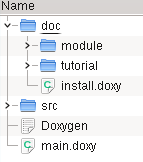
\includegraphics[width=0.4\textwidth]{image/doc-struct}
    \caption[ساختار مورد نیاز برای ایجاد مستند تکنیکی]
    {
      ساختار مورد نیاز برای یک مستند تکنیکی. هماگونه که در این تصویر قابل مشاهده
      است یک مسیر به نام \lr{doc} ایجاد می‌شود و مستندهای جانبی در آن قرار
      می‌گیرد. دیگر مستندها در متن برنامه نوشته می‌شود.
    }
    \label{standard/where-what/doc-struct}
  \end{figure}


%
% حق نشر 1390-1402 دانش پژوهان ققنوس
% حقوق این اثر محفوظ است.
% 
% استفاده مجدد از متن و یا نتایج این اثر در هر شکل غیر قانونی است مگر اینکه متن حق
% نشر بالا در ابتدای تمامی مستندهای و یا برنامه‌های به دست آمده از این اثر
% بازنویسی شود. این کار باید برای تمامی مستندها، متنهای تبلیغاتی برنامه‌های
% کاربردی و سایر مواردی که از این اثر به دست می‌آید مندرج شده و در قسمت تقدیر از
% صاحب این اثر نام برده شود.
% 
% نام گروه دانش پژوهان ققنوس ممکن است در محصولات دست آمده شده از این اثر درج
% نشود که در این حالت با مطالبی که در بالا اورده شده در تضاد نیست. برای اطلاع
% بیشتر در مورد حق نشر آدرس زیر مراجعه کنید:
% 
% http://dpq.co.ir/licence
%
\section{پیکره بندی}
در این قسمت به بررسی پرونده پیکر بندی مورد نیاز برای ایجاد مستن خواهیم پرداخت
در این پرونده علاوه بر این که تنظیمات اولیه مورد نیاز برای ایجاد مستند وجود
دارد چگونگی ایجاد مستند نیز به صورت کامل تشریح می‌شود. همواره فرض می‌شود که هر
پروژه یا قطعه در یک پروژه به صورت کامل در یک پوشه هم نام با آن قرار دارد. تمام
قطعه‌ها و پروژه‌هایی که با هم دیگر یک پروژه کلی را ایجاد می‌کنند نیز کنار یک
دیگر و در یک پوشه قرار می‌گیرند.

مستند تکنیکی ایجاد شده از سیستم نیز خود یک زیر پروژه از پروژه کلی در نظر گرفته
می‌شود از این رو باید یک پوشه، در پوشه پروژه اصلی در نظر گرفت. این پوشه را
همواره با نام \lr{doc} در نظر می‌گیریم. مستند تکنیکی هر زیر پروژه باید به صورت
یک پرونده هم نام با همان زیر پروژه در پوشه \lr{doc} ایجاد شود. برای نمونه فرض
کنید که در پروژه اصلی سه زیر پروژه به نام‌های \lr{GUI}، \lr{Shell} و \lr{LIB}
وجود دارد. در این صورت در این پروژه یک پوشه دیگر به نام \lr{doc} باید ایجاد
و معادل با هر زیر پروژه در آن یک پوشه ایجاد شود. در شکل
\ref{wher-what-config-example-1} ساختار مورد نیاز برای این پروژه نمایش داده
شده است.

در گام بعد در هر پروژه یک پرونده پیکره بندی برای مستند فنی به نام \lr{Doxygen}
ایجاد می‌شود که داده‌های مورد نیاز برای ایجاد مستند در آن قرار خواهد گرفت. در
شکل \ref{wher-what-config-example-1} محل قرار گرفتن پرونده‌های پیکره بندی نشان
داده شده است. از آنجا که محل خروجی مستندهای ایجاد شده بر اساس تنظیم‌های موجود
در همین پرونده‌های تعیین می‌شود باید خصوصیت مسیر خروجی برای هر مستند را به
گونه‌ای اصلاح کرد که مستندهای ایجاد شده در مسیر مناسب قرار گیرد. برای نمون در
پرونده پیکربندی پروژه \lr{GUI} مسیر خروجی به صورت زیر اصلاح می‌شود:

\begin{latin}
\lstset{language=bash}  
\begin{lstlisting}[frame=single] 
OUTPUT_DIRECTORY       = ../doc/GUI
INPUT                  = ./
\end{lstlisting}
\end{latin}

همانگونه که در نمونه آورده شده قابل مشاهده است علاوه بر مسیر خروجی باید مسیر
ورودی پروژه را نیز تعیین کرد. از آنجا که برای هر پروژه به صورت جداگانه یک پرونده
پیکره بندی ایجاد می‌شود کافی است که مسیر ورودی را مسیر جاری قرار داد. با این
تنظیم بدون ترس از محل قرار گرفتن مستند‌ها می‌توان به سادگی در پایان پروژه مستند
فنی را بر اساس تمام پروژه‌ها موجود در پروژه اصلی ایجاد کرد. این فرآیند می‌تواند
به صورت خودکار در پروژه‌های بزرگ انجام شود.

مستندگر \lr{Doxygen} تنها مسیر ورودی تعیین شده را برای یافتن پرونده‌های ورودی
جستجو می‌کند، در صورتی که ساختار تشریح شده برای مستندها و برنامه‌ها به صورت
سلسله مراتبی در نظر گرفته شده است. در این حالت در پرونده پیکره بندی باید جستجوی
بازگشتی برای یافتن پرونده‌ها فعال شود. برای فعال کردن این روش جستجو باید تنظیم
زیر را در پرونده پیکره بندی اضافه کرد:

\begin{latin}
\lstset{language=bash}  
\begin{lstlisting}[frame=single] 
FILE_PATTERNS          = *.h \
                         *.hh \
                         *.hxx \
                         *.hpp \
                         *.h++ \
                         *.dox \
                         *.doxy

RECURSIVE              = YES
\end{lstlisting}
\end{latin}

همانگونه که در کده بالا قابل مشاهده است علاوه بر فعال کردن جستجوی بازگشتی،
می‌بایست ساختارها و پرونده‌هایی که باید به عنوان ورودی قرار گیرد را تعیین کرد.
گرچه که پرونده‌های ورودی وابسته بر اساس نوع پروژه و زبان‌های برنامه سازی به کار
گرفته شده در آن تعیین می‌شود، اما در هر حال پرونده‌های با پسونده \lr{*.doxy}
باید همواره به عنوان ورودی مورد استفاده قرار گیرد.

علاوه بر تمام خصوصیت‌هایی که در این بخش مورد بررسی قرار گرفت خصوصیت‌های دیگری
نیز وجود دارد که باید در یک پرونده پیکرده بندی تعیین شوند. در کد زیر  برخی از
مهم‌ترین تنظیم‌های مورد نیاز برای یک پروزه آورده شده است:

\begin{latin}
\lstset{language=bash}  
\begin{lstlisting}[frame=single] 
DOXYFILE_ENCODING      = UTF-8
PROJECT_NAME           = My Project GUI
PROJECT_NUMBER         = 0.1.0 beta
PROJECT_BRIEF          = MGUI
PROJECT_LOGO           = ./images/logo.png
\end{lstlisting}
\end{latin}

در نهایت با ایجاد تنظیم‌های مورد نیاز برای تمام پروژه‌ها می‌توان به سادگی مستند
فنی مورد نیاز برای پروژه را ایجاد و در موقع نیاز از آنها استفاده کرد.

%
% حق نشر 1390-1402 دانش پژوهان ققنوس
% حقوق این اثر محفوظ است.
% 
% استفاده مجدد از متن و یا نتایج این اثر در هر شکل غیر قانونی است مگر اینکه متن حق
% نشر بالا در ابتدای تمامی مستندهای و یا برنامه‌های به دست آمده از این اثر
% بازنویسی شود. این کار باید برای تمامی مستندها، متنهای تبلیغاتی برنامه‌های
% کاربردی و سایر مواردی که از این اثر به دست می‌آید مندرج شده و در قسمت تقدیر از
% صاحب این اثر نام برده شود.
% 
% نام گروه دانش پژوهان ققنوس ممکن است در محصولات دست آمده شده از این اثر درج
% نشود که در این حالت با مطالبی که در بالا اورده شده در تضاد نیست. برای اطلاع
% بیشتر در مورد حق نشر آدرس زیر مراجعه کنید:
% 
% http://dpq.co.ir/licence
%
\section{برگه نخست}
  برگه نخست ابتدایی ترین قسمت در یک مستند است، از این جهت در ایجاد و سازمان دهی
  یک مستند بسیار مهم است.
  اگر این صفحه به درستی و به شیوه مناسب طراحی و ایجاد نشده باشد، خواننده مستند
  نمی‌تواند به سادگی مستند را مور استفاده قرار دهد و در نخستین برخورد دچاد
  سردرگمی خواهد شد.

  پیش از هر چیز باید به این نکته اشاره کرد که برگه عبارت است از یک بخش از مستند
  که در حالت کلی معادل با یک گفتار در یک کتاب است.
  هر برگه را در یک پرونده \lr{*.doxy} ایجاد می‌شود و در آن متن برگه به صورت کامل
  نوشته می‌شود.
  هر برگه همانند یک گفتار می‌تواند از بخشهای متفاوتی ایجاد شده باشد.
  هر بخش و زیر بخشهای آن نیز به صورت منظم و پشت سرم هم در پرونده برگه نوشته
  می‌شود. در کد زیر نمونه‌ای از یک برگه آورده شده است.
  
\begin{latin}
\lstset{language=C++}
\begin{lstlisting}[frame=single] 
/**
\page pageid Page Title
  Page Body.
  
  \section sectionid Section Title
    Section Body.

    \subsection subsectionid Subsection Title
      Subsection Body.
*/
\end{lstlisting}
\end{latin}

  همانگونه گه پیش از این نیز گفته شد، برگه نخست ابتدایی ترین قسمتی از مستند است
  که هر خواننده با آن روبرو می‌شود. بی شک انتخاب دقیق مطالب مورد نیاز و
  ساختاردهی آن در تاثیر پذیری آن اثر خواهد داشت.
  در نخستین قسمت از برگه نخست باید به معرفی نرم افزار و بیان اهداف اصلی طراحی و
  ایجاد آن اختصاص داده شود.
  هر خواننده با دانستن اهداف یک نرم‌افزار یا بسته نرم‌افزاری می‌تواند به چرایی
  بسیاری از رویکردهای سیستم پاسخ دهد.
  دور از ذهن نیست که برای انجام هر پردازش ویا اجرای هر فرآیند در یک سیستم
  نرم‌افزاری روش‌های متفاوتی وجود داشته باشد. برای نمونه در ذخیره و بازیابی
  داده‌های می‌توان از روش‌های متفاوتی چو پایگاه داده‌ها، پرونده‌های متنی و
  باینری و یا بسیاری از روش‌های دیگر استفاده کرد. واضح است که خواننده با اشراف
  بر اهداف یک سیستم می‌تواند به راحتی درک کند که چرا در یک مسئله از روشی خاص
  استفاده شده است و در نتیجه توانایی و محدودیت سیستم در کجا است.

  در توسعه یک سیستم مدیران پروژه در نخستین گام به دنبال سیستم‌های موجودی خواهند
  بود که بتواند تمام اهداف مورد نظر آنها را پوشش دهد. در بسیاری از موارد نیز
  اهداف و نیازهای سیستم مورد بازبینی قرار گرفته و گه گاه از آنها کاسته می‌شود تا
  کاملا با اهداف یک سیستم موجود هم سو شود. در این صورت ابتدایی ترین پرسش مطرح
  برای یک مدیر اهداف یک سیستم ایجاد شده است. بر این اساس ایجاد یک بخش مجزا و
  تشریح اهداف یک سیستم بسیار اساسی به نظر می‌رسد.

  شکی نیست که پیش از هرچیز در یک مستند تکنیکی باید سیستم را به صورت کامل تعریف
  کرد و اهداف مورد نظر در طراحی و پیاده سازی آن را تشریح کرد اما علاوه بر این
  نیاز است که ساختار مستند نیز به صورت کامل تشریح شود. این تصور اشتبا است که
  همواره هر خواننده از ابتدایی ترین موضوع در مستند شروع کرده و تا انتها تمام
  ستند را به ترتیب مطالعه خواهد کرد.
  خوانندگان یک مستند با دیدگاهی متفاوت تنها به دنبال دسته‌ای خاص از اطلاعات
  ایجاد شده در یک مستند هستند و از خواندن بسیار از بخشهای مستند صرف نظر خواهند
  کرد. در این حالت معرفی مفید و کامل ساختار مستند می‌تواند بسیار مفید واقع شود و
  احساس خوبی را در خوانندگانی که برای اولین بار مستند را مطالعه می‌کنند ایجاد
  کند.

  مدیران  سیستم‌های نرم افزاری در فرآیند گزینش یک سیستم جدید در پی داده‌های چون
  سخت‌افزارهای مورد نیاز، وابستگی به بسته‌های نرم‌افزاری دیگر، قابلیت انتقال به
  روی سکوی‌های متفاوت و دیگر اطلاعات از یک سیستم موجود هستند. این در حالی است که
  توسعه دهندگان سیستم‌های نرم افزاری بیشت به دنبال اطلاعاتی در زمینه به کار گیری
  سیستم در کاربردهای مورد نظر هستند. اینها تنها بخشی از خوانندگان با دیدهای
  متفاوت هستند که مستند تکنیکی سیستم‌های موجود را مورد بررسی و مطالعه قرار
  می‌دهد. در چنین شرایطی ایجاد ساختار مناسب در مستندها و تشریح کافی و کامل آن
  می‌تواند خوانندگان را در یافتن اطلاعات مورد نظرشان از یک سیستم موجود یاری کند.

  سومین بخش از برگه نخست مستند که باید در نظر گرفته شود، بیان سطوح متفاوت موجود
  در یک مستند و توصیه‌های مناسب برای خوانندگان مستند است. بی شک مستند یک سیستم،
  به خصوص زمانی که اندازه سیستم بزرگ است، زمینه‌های متفاوتی را پوشش داده و در
  نتیجه خوانندگان متفاوتی را به خود خواهد دید از این رو تعیین زمینه‌های متفاوت
  موجود و توصیه مناسب به خوانندگانی که قصد مطالعه مستند را دارند می‌تواند آنها
  را در یافتن مناسب اطلاعات مورد نیازشان یاری کند. در کد نمونه‌ای که در ادامه
  آورده شده است یک ساختار ابتدایی برای برگه نخست مستند ارائه شده است.
\begin{latin}
\lstset{language=C++}
\begin{lstlisting}[frame=single] 
/**
\mainpage
  Introduction

\section docstruct Document Structuer
  Document Struction

\subsection whoread Who Read
  Who Read

\section whatsnew New
  What is New

\section bugs Closed Bugs
  Bugs
*/
\end{lstlisting}
\end{latin}

  همان گونه که در متن مستند نوشته شده قابل مشاهد است، دو بخش جدید نیز در انتهای
  برگه نخست پیش بینی شده است.
  اولین بخش در مورد توانایی‌های جدیدی است که به نسخه جدید از سیستم اضافه شده است
  در حالی که دومین بخش در مورد خطا‌هایی است که از نسخه پیشین حذف شده است. این دو
  بخش در رابطه با سیستم‌هایی است که دورده زمانی زیادی را دارند و در نسخه‌های
  متفاوت توسعه می‌یابند.

  
%
% حق نشر 1390-1402 دانش پژوهان ققنوس
% حقوق این اثر محفوظ است.
% 
% استفاده مجدد از متن و یا نتایج این اثر در هر شکل غیر قانونی است مگر اینکه متن حق
% نشر بالا در ابتدای تمامی مستندهای و یا برنامه‌های به دست آمده از این اثر
% بازنویسی شود. این کار باید برای تمامی مستندها، متنهای تبلیغاتی برنامه‌های
% کاربردی و سایر مواردی که از این اثر به دست می‌آید مندرج شده و در قسمت تقدیر از
% صاحب این اثر نام برده شود.
% 
% نام گروه دانش پژوهان ققنوس ممکن است در محصولات دست آمده شده از این اثر درج
% نشود که در این حالت با مطالبی که در بالا اورده شده در تضاد نیست. برای اطلاع
% بیشتر در مورد حق نشر آدرس زیر مراجعه کنید:
% 
% http://dpq.co.ir/licence
%
\section{برگه‌های دیگر}
  علاوه بر برگه نخست برگه‌های دیگری نیز در مستند وجود دارند که جنبه‌های متفاوتی
  از سیستم را مورد بررسی قرار می‌دهند. نصب و راه اندازی، مبانی مورد استفاده در
  سیستم، به کارگیری و خطاهای متداول سیستم تنها بخشی از مستندهایی است که معمولا
  در یک مستند تکنیکی وجود دارد.

  به این نکته باید توجه داشت که در یک مستند تکنیکی دو جنبه کاملا مجزا و در عین حال
  تاثیر گذار وجود دارد: ساختار و سازماندهی مستندها. ساختار
  مستند (همانگونه که در بخش پیش به آن اشاره شد) به چینش و ترتیب مستندهای ظاهر
  شده در متن مستند گفته می‌شود. بخش‌ها زیر بخش‌ها گفتارها و جنبه‌هایی از سیستم که باید 
  مور بررسی قرار گیرد همگی موضوعاتی هستند که در ساختار دهی مستند مورد توجه قرار می‌گیرند.
 این درحالی است که سازمان
  دهی مستند فرآیندی است که در آن قرار دادن مستندها در مسیرهای مشخص، تعیین نام پرونده‌ها و مدیریت
  مستند ایجاد شده پرداخته می‌شود.

  برای نمونه این که تمام مستندهای جانبی باید در مسیر \lr{doc} قرار گیرد و با پسوند
  \lr{*.doxy} ذخیره شود به سازماندهی مستند است در حالی که معرفی سیستم و
  تشریح اهداف آن به ساختار مستند مربوط می‌شود.
  در طراحی مستند مناسب باید به هر دو جنبه مورد توجه باشد، از این رو در این بخش هر دو
  جنبه مورد بررسی قرار خواهد گرفت. از انجا که تعیین یک مرز کاملا مشخص بین این
  دو دشوار و در برخی موارد منجر به پیچیده شدن موضوع می‌شود هر دو آنها باهم مورد بررسی قرار خواهد گرفت.

  هر برگه معادل با یک فصل در نظر گرفته خواهد شد که در یک پرونده جدا با پشوند
  \lr{*.doxy} ایجاد می‌شود. از این رو برگه‌ها نیز باید در مسیر دیگر مستندهای
  جانبی یعنی در پوشه \lr{doc} قرار بگیرند.
  هر بخش با استفاده از برچسب \lr{page} در مستند مشخص شده که با استفاده از یک
  شناسه در کل مستند قابل آدرس دهی است.
  از آنجا که شناسه هر برگه منحصر به فرد است، استفاده از شناسه برگه به عنوان نام
  پرونده نه تنها مشکل نام گذاری پرونده‌ها را حل می‌کند بلکه منجر به دستیابی راحت
  به برگه‌ها در زمان توسعه مستند می‌شود. با این روش به سادگی و تنها با مشاهده
  نام پرونده می‌توان از مطالب درون آن اطلاع یافت.

  یک برگه می‌تواند به عنوان یک زیر بخش و یک زیر برگه از یک برگه دیگر در نظر
  گرفته شود (اضافه کردن یک برگه به عنوان زیربرگ در برگه دیگر با استفاده از برچسب
  \lr{subpage} انجام می‌شود که شرح کامل آن در بخش بسته بندی مستند آمده است).

  زمانی که تعداد زیربرگه‌های یک برگه زیاد می‌شود بهتر است که آنها را در یک پوشه
  جدا ( و هم نام با شناسه برگه) قرار داد. اما اگر تعداد زیر برگه‌ها کم باشد
  می‌توان آنها را در انتهای پرونده برگه اصلی اضافه کرد. مستند زیر یک نمونه از
  ایجاد برگه و زیر برگه‌ها در یک پرونده را نشان می‌دهد.

\begin{latin}
\lstset{language=C++}
\begin{lstlisting}[frame=single]
/**
\page pageid Example
  Page budy
  ....
  \subpage subpageid1
  \subpage subpageid2
  ....
*/
/**
\page subpageid1 Subpage Title 1
...
*/
....
\end{lstlisting}
\end{latin}

  مناسب ترین روش، ایجاد برگه‌های اصلی در مسیر \lr{doc} و ایجاد زیر برگه‌ها هر یک در زیر
  پوشه‌های مجزا به ازای هر برگه اصلی است - برگه اصلی در اینجا به معنی برگه‌هایی
  است که به عنوان زیر برگ هیچ برگ دیگر از مستند نباشد.

  تعیین برگه‌های اصلی مورد نیاز در هر مستند دشوار است و بسته به اندازه و نوع
  پروژه می‌تواند بسیار متفاوت باشد. اما دسته‌ای از این برگه‌ها
  تقریبا در تمام مستندهای تکنیکی وجود دارند.
  در فهرست زیر پر کاربرد ترین برگه‌های موجود در مستندهای تکنیکی آورده شده است:
  \begin{itemize}
   \item نصب و راه اندازی
   \item مبانی
   \item کاربردها
   \item پرسشهای متداول
  \end{itemize}
  در ادامه این بخش، این برگه‌ها به صورت مفصل‌تر مورد بررسی قرار  خواهد گرفت.

  
  
\subsection{نصب و راه اندازی}
  راهنمای نصب یک نرم‌افزار در بسیاری از موارد با راهنمای مدیریت و کاربری یک
  سیستم نرم افزاری و یا سخت افزاری هم پوشانی دارد. این هم پوشانی به دلیل وجود
  تنظیم‌های مورد نیاز در فرآیند نصب است که به عنوان حالت اولیه سیستم در نظر
  گرفته می‌شود.

  نصب و راه اندازی سیستم با تنظیم و به کارگیری آن در رابطه است و
  گاه شامل اطلاعاتی می‌شود که در مستندهای دیگر مانند مستند مدیریت و یا کاربری 
  هم پوشانی دارد. در این شرایط مناسب است که به مستندهای دیگر ارجاع داده شده و از
  ذکر دوباره اطلاعات خوداری کرد. اما باید به این نکته توجه داشت که بیان دوباره
  نکته‌های مهم می‌تواند در مستقل شدن مستند و نصب سریع و آسان سیستم کمک کند. به
  هر حال نباید از زیاده گویی و افزونگی مستند غافل شد.

  موارد متفاوتی وجود دارد که در این بخش باید به صورت کامل به آن پرداخته شود. در
  اینجا برخی از موارد لاز در فرآیند نصب و راه اندازی سیستم بیان و 
روش مستندسازی آنها مورد بررسی قرار گرفته شده است.


\paragraph{پیش نیازها}
   چه نوع نرم‌افزار، سخت افزار، و یا سکوی نرم‌افزاری برای نصب یک سیستم مورد نیاز
   است؟ آیا سیستم به روی هر سکوی نرم افزاری و یا سخت افزاری قابل اجرا است؟ آیا
   سیستم با سیستم‌های عامل متفاوت چون لینوکس، مک، و یا ویندوز سازگار است؟
   پردازشگر مورد نیاز سیستم چه قابلیت‌هایی باید داشته باشد؟ اینها بخشی از
   پرسش‌هایی است که باید در این بخش به آن پرداخته شود.

   توجه به این نکته بسیار مهم است که پیش‌نیازهای یک سیستم گاهی از خود آن نیز
   مهم‌تر می‌شود. برای نمونه حالتی را تصور کنید که در آن سیستم به صورتی ایجاد
   شده است که تنها به روی یک سیستم عامل خاص قابل اجرا است در این صورت فرد یا
   گروهی که به آن سیستم عامل دسترسی ندارند نمی‌توانند از این سیستم استفاده کنند.
   پیش‌نیازهای یک سیستم در انتخاب یک سیستم بسیار موثر خواهد بود.

   به عنوان نمونه در راهنمای نصب سیستم عامل ویندوز ویستا، موارد زیر به عنوان
   پیش‌نیاز نصب سیستم معرفی شده است:
\begin{config}
1 GHz 32-bit (x86) or 64-bit (x64) processor
512 MB of system memory
20 GB hard drive with at least 15 GB of available space
Support for DirectX 9 graphics and 32 MB of graphics memory
DVD-ROM drive
Audio Output
Internet access
\end{config}
   بر اساس این پیش‌نیازها کاربران و مدیران می‌توانند سیستم مورد نیاز
   خود را بر اساس پیش‌نیاز آنها انتخاب کنند. گرچه یک سیستم ایده آل سیستمی است که پیش‌نیازهای آن کم و
   با هر شرایطی سازگار باشد اما در هر حال باید پیش‌نیاز سیستم به درستی تعیین شده
   باشد تا کاربران در فرآیند نصب و راه اندازی سیستم با مشکل روبرو نشوند.
   
\paragraph{دست یابی به سیستم}
  پیش از هر کاری نیاز است که کاربران به نرم‌افزار و یا کد منبع آن دست پیدا کنند.
  در این بخش بر اساس توافق نامه یک نرم‌افزار به کاربران اطلات لازم جهت دست یابی
  که نرم افزار داده می‌شود. برای نمونه در سیستم های متن باز به کاربران آموزش
  داده می‌شود که چگونه با استفاده از مدیریت نسخه‌ها به یک نسخه خاص از کد منبع
  نرم‌افزار دست پیدا کنند.
  
\paragraph{تنظیم و نصب سریع}
   گاهی در مستند‌های فنی از این بخش به عنوان شروع سریع یاد می‌کنند که در آن
   فرآیند نصب و به کارگیری عملی سیستم با کمترین تنظیم و منابع تشریح می‌شود. به
   کارگیری ساده و سریع یک سیستم می‌تواند اعتماد کاربران را به سیستم افزایش دهد.

   در این بخش پیش شرط‌های مورد نیاز برای نصب، حالت نرم‌افزار و سخت‌افزارهای مورد
   استفاده و درک لازم از حالت سیستم به صورت کامل تشریح شده و کاربر برای نصب
   مقدماتی سیستم آماده می‌شود. علاوه بر این در این بخش عبارت‌ها و واژگان جدید
   مطرح در سیستم که حالت و یا قسمت خاصی از سیستم را تشریح می‌کند به صورت کامل
   بیان می‌شود.

   روش مناسب برای تعیین درک کامل از سیستم، تشریح سیستم و ساختار آن با
   استفاده از نمودارها است.
   ساختار سیستم، واسطه‌های مورد حمایت، شبکه‌های مورد استفاده و بسیاری دیگر از
   اجزای مورد نیاز سیستم را می‌توان با استفاده از یک نمودار به سادگی تشریح
   کرد و درک کاملی را از سیستم و پیش‌نیازهای آن به وجود آورد. درک سیستم نه تنها
   فرآیند نصب را قابل درک کرده بلکه کاربران را در تعیین و رفع مشکلات سیستم یاری
   می‌کند. در شکل 
   \ref{تصویر-ساختار-خوشه-پایگاه-داده}
    یک نمونه از شکل‌های مورد
   استفاده در راهنمای نصب یک سیستم نرم‌افزاری نمایش داده شده است.
  \begin{figure}
    \centering
    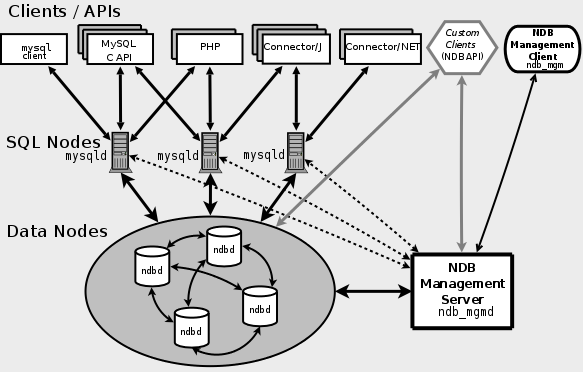
\includegraphics[width=0.75\textwidth]{image/mysql-cluster-install.png}
    \caption[ساختار خوشه‌ای پایگاه داده]
    {
      در این تصویر ساختار خوشه‌ای \lr{MySQL} نمایش داده شده است. بر اساس این
      ساختار کاربران می‌توانند پیش نیازهای سیستم را در نصب خوشه‌ای و تفاوت آن را
      با دیگر روش‌های نصب در این نرم افزار درک کند.
      از این شکل در راهنمای نصب این نرم‌افزار استفاده شده است.
    }
    \label{تصویر-ساختار-خوشه-پایگاه-داده}
  \end{figure}
  
   کاربران سیستم در اولین برخورد و مبتنی بر مستندهای این بخش است که قادر خواهند بود
   سیستم را به صورت عملی نصب کرده و به کار ببرند. لذا طراحی و نوشتن مناسب این بخش
   می‌تواند در جلب اعتماد کاربران بسیار مفید باشد. به این نکته توجه داشته باشید
   که زمانی یک کاربر به سیستم اعتماد کند آن را به کار خواهد بست و در ادامه
   تنظیم‌های پیشرفته سیستم را نیز فرا خواهد گرفت. پژوهشها نشان می‌دهد که عدم
   توانایی نصب راحت و به کار گیری یک سیستم منجر به کاهش علاقه کاربران در به
   کارگیری سیستم خواهد شد از این رو پرداختن به این بخش می‌تواند بسیار مهم باشد.

\paragraph{آزمون و خطایابی}
    تمام سیستم‌های نرم‌افزاری و سخت‌افزاری از روش‌های متفاوتی برای نمایش حالت
    درونی سیستم استفاده می‌کنند.
    واسطه‌ها گرافیکی، پیام‌های صوتی تصویری، دریچه‌های محاوره‌ای بخشی از روکردهای
    مورد استفاده در نمایش حالت درونی یک سیستم نرم‌افزاری است. سیستم‌های
    نرم‌افزاری با استفاده از همین رویکردها رویدادهای داخلی سیستم را به
    کاربران گزارش می‌کنند.

    در این بخش باید به صورت کامل به خطاهای احتمالی در فرآیند نصب یک نرم‌افزار
    پرداخته شده و راه مناسب رفع آنها به صورت کامل تشریح شود. اطلاعات موجود در
    این بخش می‌تواند کاربران را در نصب و راه‌اندازی راحت سیستم یاری کند.

    برای نمونه فرض کنید که سیستمی فیزیکی وجود دارد و در جلو آن چراغی با چهار
    رنگ قرار تعبیه شده است.
    این سیستم با استفاده از رنگهای متفاوت این چراغ‌ها حالت درونی خود را به کاربران
    سیستم گزارش می‌کند.
    از این رو در این بخش از مستند به تشریح مفهوم رنگ‌های متفاوت و روش برخورد با هر 
یک بیان می‌شود. برای نمون چراغ قرمز به معنی مناسب نبودن
    منبع تغذیه است که در این صورت باید سیستم خاموش شده و منبع تغذه آن تعمیر شود.

    تشریح روش‌های مناسب آزمون سیستم بعد از نصب نیز یکی دیگر موضوعاتی است که در
    این بخش به آن پرداخته می‌شود. اطمینان از نصب بودن و درستی حالت درونی یک
    سیستم برای استفاده عملی از آن بسیار اساسی است.

\paragraph{به روز رسانی}
    علاوبه بر نصب یک سیستم نرم‌افزاری به روز رسانی آن نیز از اهمیت زیادی
    برخوردار است. کاربران باید به صورت کامل از فرآیند به روز رسانی سیستم آگاه
    بوده و بتواند سیستم را به روز کند.

    محدودیت‌های به روز رسانی و یا توافق نامه‌های مورد نیاز در به روز رسانی
    باید در این بخش مورد بررسی قرار گیرد. کاربران بر اساس این توافق نامه
    می‌توانند در مورد استفاده یا عدم استفاده از یک بسته نرم‌افزاری تصمیم بگیرند.
    
\subsection{مبانی}

مبانی در اینجا، آن دسته از دانش‌های فنی است که نرم‌افزار مبتنی بر آنها توسعه یافته است.
برای نمونه می‌توان بسته‌های متفاوتی نام برد که بر اساس مبانی خاص ریاضی توسعه یافته‌اند
و در کاربردهای خاص مورد استفاده قرار می‌گیرند. مبانی مورد استفاده باید به صورت کامل و روشن
بیان شود تا نه تنها توسط تیم توسعه در آیند، بلکه کاربران سیستم مورد استفاده قرار گیرد.

حجم مستند مبانی ممکن است از یک صفحه تا چندین بخش قابل متغییر باشد، اما نکته‌ای که باید در نوشتن
مبانی مورد توجه قرار گیرد بیان کامل و روشن تمام مبانی مورد استفاده است. این نکته به ویژه زمانی
که نظریه‌های متفاوتی در راستای اهداف پروژه وجود دارد و تمییز بین این نظریه‌ها از اهمیت
ویژه‌ای برخوردار است، پر اهمیت می‌شود.
  
\subsection{کاربردها}
بی شک هر سیستم بر اساس اهداف از پیش تعریف شده‌ای سازمان دهی و پیاده‌سازی می‌شود. اهداف سیستم 
در بسیاری از موارد منجر به ایجاد بسیاری از محدودیت‌ها در سیستم پیاده‌سازی شده خواهد شد، از این
رو لازم است که نه تنها تمام کاربردهای نرم‌افزار بلکه محدودیت‌های آن نیز به صورت کامل بیان شود.
در این بخش تمام کاربردهای و محدودیت‌های سیستم بیان و به صورت کامل مورد بررسی قرار خواهد گرفت.
  
\subsection{پرسشهای متداول}
نمی‌توان تصور کرد که مستند ایجاد شده برای یک سیستم به صورت کامل واضح و کامل است. بسیاری از کاربران
طی استفاده از سیستم‌ها با پرسش‌های روبرو می‌شوند که به خوبی می‌تواند کاستی‌های مستندهای موجود را بیان 
می‌کند. در این برگه متداول‌ترین پرسش‌های مطرح در بین کاربران تعیین و به صورت کامل پاسخ داده می‌شود
تا به واضح‌تر شدن مستند فنی و کاربردهای نرم‌افزار بیفزاید.
  
\subsection{پیمان نامه‌ها}
مهم‌ترین قسمت یک مستند فنی، پیمان‌نامه آن است. در این قسمت از مستند به صورت کامل محدودیت‌های نرم‌افزار
ایجاد شده از نظر حقوقی بیان می‌شود که در انتخاب و به کارگیری هر سیستمی مهم است. گروه‌های متفاوت
از پیمان نامه‌های متفاوت استقبال و نرم‌افزارهای مورد نیاز خود را بر اساس همین پیمان نامه‌ها 
انتخاب می‌کنند.
  


%
% حق نشر 1390-1402 دانش پژوهان ققنوس
% حقوق این اثر محفوظ است.
% 
% استفاده مجدد از متن و یا نتایج این اثر در هر شکل غیر قانونی است مگر اینکه متن حق
% نشر بالا در ابتدای تمامی مستندهای و یا برنامه‌های به دست آمده از این اثر
% بازنویسی شود. این کار باید برای تمامی مستندها، متنهای تبلیغاتی برنامه‌های
% کاربردی و سایر مواردی که از این اثر به دست می‌آید مندرج شده و در قسمت تقدیر از
% صاحب این اثر نام برده شود.
% 
% نام گروه دانش پژوهان ققنوس ممکن است در محصولات دست آمده شده از این اثر درج
% نشود که در این حالت با مطالبی که در بالا اورده شده در تضاد نیست. برای اطلاع
% بیشتر در مورد حق نشر آدرس زیر مراجعه کنید:
% 
% http://dpq.co.ir/licence
%
\section{مستند پیاده سازیی}
همان گونه که پیش از نیز بیان شد، علاوه بر مستند فنی دسته‌ای دیگر از مستندها وجود دارد که در مورد 
پیاده سازی سیستم است. در این مستند برخلاف مستند فنی به روش مورد استفاده در پیاده سازی متدها و 
الگوریتم‌ها ذکر می‌شود تنها در توسعه سیستم مورد استفاده است. گرچه مستند پیاده سازی از اهمیت ویژه‌ای
برخوردار است، با این وحود نباید در مستند فنی ظاهر شود.

فرض کنید که یک توسعه دهنده سیستم در زمان پیاده سازی به یک ایده جدید در مورد پیاده سازی سیستم 
رسید است. این ایده یک مستند بسیار مهم است که باید در سیستم نگه داشته شود (تا جایی که بسیاری
از متدلوژی‌ها بر اساس این ایده‌ها سازمان‌دهی می‌شوند). مستندهای از این دست، کاملا در مورد پیاده‌سازی
سیستم است از این رو کاربردی برای کاربران سیستم ندارند.

مستندهای پیاده سازی در لابلای کدها نوشته می‌شود و از ساختار سازمان یافته‌ای همانند مستند فنی برخوردار
نیستند. گرچه چگونگی نوشتن مستند پیاده سازی کاملا شخصی است با این وجود دسته‌ای از استاندارهای برای سازمان
دهی آن وچود دارد که در ادامه به آن پرداخته خواهد شد.
مستند پیاده سازی به دو روش در برنامه‌ها بیان می‌شود: چند و تک خطی. زمانی که مستند پیاده سازی طولانی
است به صورت چند خط نوشته می‌شود این مستند به صورد زیر نوشته می‌شود:
 
\begin{latin}
\lstset{language=C++}
\begin{lstlisting}[frame=single] 
/*
 * Implementation document
 * this document is structed in multi line.
 */
\end{lstlisting}
\end{latin}

البته مستندهای کوتاه تنها در یک خط و به صورت زیر در متن برنامه‌ها نوشته می‌شود:

\begin{latin}
\lstset{language=C++}
\begin{lstlisting}[frame=single] 
// Implemtnation Doceumtn
\end{lstlisting}
\end{latin}

هر قسمت مستند که به صورت یکی از دو روش بالا در متن برنامه‌ها نوشته شود به عنوان یک مستند پیاده سازی
در نظر گرفت شده و در مستند فنی تولید شده وارد نخواهد شد.

\subsection{برچسب‌های مستند پیاده‌سازی}
فرض کنید که یک گروه پیاده‌سازی می‌خواهد با استفاده از یک ماشین برنامه ایجاد شده را به صورد کامل
بررس کرده و بر اساس آن پیام‌های مناسبی را در جهت بهبود و گسترش سیستم، ایجاد کند. بی شک این ماشین
باید مستندهای پیاده سازی را بررسی کرده و پیام‌های خود را مبتنی بر آنها ایجاد کند. برای نمونه انتظار
می‌رود که برنامه تعیین کند که کدام قسمت‌ها از برنامه ایجاد شده نیاز به بازنویسی، بهبود و یا حذف شدن 
دارد تا بتواند در فرآیند توسعه مورد استفاده قرار گیرد. بی شک این ماشین بدون در نظر گرفتن استاندارهای
مناسب برای نوشتن مستند پیاده سازی نمی‌تواند پیام‌های مناسبی را ایجاد کند. در این قسمت یک ساختار ابتدایی
برای نوشتن مستند پیاده سازی تشریح خواهد شد که می‌تواند این فرآیند را به صورت کامل پوشش دهد.

برخلاف مستند فنی، در مستند پیاده‌سازی تنها تعداد محدودی برچسب موجود است که برای ساختاردهی مستند مورد
استفاده قرار می‌گیرد. این برچسب‌ها باید هموار در ابتدای نخستن خط از هر بسته مستند پیاده سازی نوشته
شده و به صورت کامل از ساختار تعریف شده پیروی کند. گرچه امکان نوشتن مستند پیاده‌سازی در چندین خط وجود
دارد اما همواره در سطر اول باید با استفاده از یک جمله به صورت کامل و شفاف هدف اصلی مستند نوشته شود.
علاوه بر این باید تعیین شود که چه فردی و در چه زمان مستند را ایجاد و یا ویرایش کرده است. مستند زیر
را در نظر بگیرد:


\begin{latin}
\lstset{language=C++}
\begin{lstlisting}[frame=single] 
/*
 * TODO : maso 1390-12 : Document title.
 * document text.
 */
\end{lstlisting}
\end{latin}

همان گونه که در این قطعه مستند قابل مشاهد است، در سطر نخست با استفاده از یک برچسب، نام توسعه دهنده، 
تاریخ و عنوان نه تنها مفاهیم کلی مستند انتقال یافته بلکه امکان ردیابی اطلاعات نیز ممکن شده است. 
برای سادگی و ایجاد تمایز میان برچسب‌های مورد استفاده در مستند فنی و پیاده سازی، برچسب‌های مورد استفاده
در مستند پیاده‌سازی را چمپ\LTRfootnote{برچسب مستند پیاده‌سازی} 
 گفته خواهد شد. ساختار کلی چمپ‌ها به صورت زیر است:


\begin{latin}
\lstset{language=C++}
\begin{lstlisting}[frame=single] 
/*
 * <TAG> : <Developer> <Date> : <Short Discription>
 * <Discription>
 */
\end{lstlisting}
\end{latin}

گاهی کل مستند فنی در یک سطر قابل بیاد است در این صورت می‌توان از مستند پیاده‌سازی تک سطری استفاده کرد.
قالب کلی این مستند نیز با استفاده از چمپ‌ها به صورت زیر است:

\begin{latin}
\lstset{language=C++}
\begin{lstlisting}[frame=single] 
//<TAG> : <Developer> <Date> : <Short Discription>
\end{lstlisting}
\end{latin}


\subsubsection{\lr{FIXME}}
این چمپ از بالاترین اولویت برخورد دارد است. زمانی که یک برنامه ناقص است و بر این اساس سیستم قابلیت
رسیدن به اهداف پیش بینی شده را ندارد از این برچسب استفاده می‌شود. به بیان دیگر هر گاه قسمتی از برنامه
نوشته نشده است و باید پیش از اتمام پروژه حتما کامل شود از این برچسب استفاده می‌شود.

\subsubsection{\lr{TODO}}
اولویت این چمپ معمولی است. زمانی که انجام یک کار در پیاده‌سازی کامل یک سیستم لازم است اما عدم انجام 
آن آسیب مهمی را به سیستم وارد نمی‌کند از این چمپ استفاده می‌شود. برای نمونه فرض کنید که ممکن است در
برخی از مواقع شبکه مورد استفاده دچار مشکل شود در این صورت باید برنامه‌ای نوشته شود که بتواند به صورت
مناسب مشکل را به کاربر انتقال دهد اما احتمال این رویداد در سیستم بسیار کم است. بنابر این می‌توان 
با استفاده از این چمپ پیاده‌سازی برنامه مناسب را به زمانی دیگر موکول کرد.

\subsubsection{\lr{WARNING}}
این چمپ از پایین‌ترین اولویت برخوردار است و تنها زمانی به کار می‌رود که نیاز به گوش زد کردن برخی از 
نکات وجود داشته باشد. برای نمونه فرض کنید که نیاز است داده‌های ورودی یک پردازش داده‌های مثبت باشند
اما بررسی این نکته که آیا تمام داده‌ها مثبت است در برنامه انجام نشده باشد (که منشا آن می‌تواند ساختار
داده‌ای موجود در سیستم باشد). اما این کار از امنیت سیستم می‌کاهد چرا که ورود یک داده نا معتبر می‌تواند
کار سیستم را متوقف کند. از این رو با استفاده از این چمپ می‌توان مشکل را با توسعه دهندگان بعد گوش زد
کرد.

\subsubsection{\lr{MINDSTORME}}
گرچه اولویت این چمپ با \lr{WARNING} برابر است اما مفهومی کاملا متفاوت دارد. فرض کنید که در طی فرآیند 
توسعه سیستم ایده‌هایی جدید برای بهبود و گسترش سیستم به وجود آید. در این صورت باید راهکاری برای 
جمع آوری این ایدها و انتقال آنها به گروهای بعدی توسعه ایجاد شود. با استفاده از این چمپ می‌توان ایده‌های
جدید برای توسعه نرم‌افزار را در خلال آن ایجاد و مدیریت کرد.



%
% حق نشر 1390-1402 دانش پژوهان ققنوس
% حقوق این اثر محفوظ است.
% 
% استفاده مجدد از متن و یا نتایج این اثر در هر شکل غیر قانونی است مگر اینکه متن حق
% نشر بالا در ابتدای تمامی مستندهای و یا برنامه‌های به دست آمده از این اثر
% بازنویسی شود. این کار باید برای تمامی مستندها، متنهای تبلیغاتی برنامه‌های
% کاربردی و سایر مواردی که از این اثر به دست می‌آید مندرج شده و در قسمت تقدیر از
% صاحب این اثر نام برده شود.
% 
% نام گروه دانش پژوهان ققنوس ممکن است در محصولات دست آمده شده از این اثر درج
% نشود که در این حالت با مطالبی که در بالا اورده شده در تضاد نیست. برای اطلاع
% بیشتر در مورد حق نشر آدرس زیر مراجعه کنید:
% 
% http://dpq.co.ir/licence
%
% در این پرونده چگونگی نوشتن مستندهای سی بیان می‌شود. این استانداردهای بر اساس
% رابطه میان ابزارهای مستند نویسی با Doxygen تعیین خواهد شد.
% مصطفی برمشوری ۱۳۹۰
\chapter{استانداردهای زبان \lr{C/C++}}

در این فصل استانداردهایی برای مستندنویسی کدهایی که به زبان \lr{C/C++} نوشته
می‌شود شرح داده شده است. تمام مواردی که در فصل‌های قبل در مورد مستندنویسی گفته
شد همگی مورد قبول است. در این قسمت نحوه استفاده از این موارد در پروژه‌هایی که به
زبان \lr{C/C++}  نوشته شده‌اند را نشان می‌دهیم. در پروژه‌هایی به این زبان
پرونده‌های سرآیند و پیاده‌سازی وجود دارد که در این قسمت گفته می‌شود که در هر بخش
از پروژه چه مستندهایی نوشته می‌شود.

\section{مستند فنی}
% FIXME : مصطفی ۱۳۹۰-۱۲ :  
% مستند فنی در پرونده‌های سرآیند نوشته می‌شود.
% تمام برچسب‌ها بر اساس استاندار Qt است تا همه را پوشش دهد

در زبان برنامه سازی سی، پرونده‌های سرآیند تنها پرونده‌هایی هستند که بدون ترجمه
انتقال داده می‌شوند. این پرونده‌ها تعیین می‌کند که در پرونده‌های باینری ایجاد
شده چه توابع و موجودیت‌هایی وجود دارد و لینکر چگونه باید پیوندهای مورد نیاز را
ایجاد کند. از آنجا که این پرونده‌ها همواره به عنوان جزئی از خروجی انتقال داده
می‌شوند بهتر است که مستندهای فنی در این پرونده‌ها نوشته شود.

نوشتن مستندهای فنی در پرونده‌های سرآیند منجر به افزایش حجم داده در زمان انتقال
محصول می‌شود. فرض کنید که پروژه‌ای ایجاد شده است، در این صورت در فرآیند انتقال
نیاز است علاوه بر محصول مستندهای تکنیکی نیز به نحوی همراه با محصول انتقال داده
شود، در این صورت مستند فنی علاوه نه تنها به صورت مستقل بلکه همراه با پرونده‌های
سرآیند وجود دارد.

گرچه درنگاه اول افزایش حجم محصول یک ایراد اساسی برای نوشتن مستندهای فنی در
پرونده‌های سرآیند به شمار می‌آید اما با این حال از دیدگاه پیاده ساز به عنوان یک
مزیت در نظر گرفته می‌شود. توسعه دهندگان یک سیستم بدون نیاز به مراجعه به کد
برنامه می‌توانند به مستند فنی آن دست پیدا کنند. بسیاری از محیط‌های مجتمع توسعه
(مانند \lr{Eclipse}) مستندهای نوشته شده در پرونده‌های سرآیند را به عنوان مستند
یک موجودیت برای کاربران نمایش می‌دهد. علاوه بر این می‌توان با استفاده از ابزارهای
مناسب پیش از ایجاد یک محصول، مستندهای فنی موجود در پرونده‌های سرآیند را از محصول
حذف کرد.

\begin{note}
گرچه تنها مستند موجود در پرونده‌های سرآیند، مستند فنی است و توسعه دهندگان سیستم
باید از نوشتن مستند پیاده سازی در این پرونده‌ها خودداری کنند، اما در صورت لزوم
می‌توان برخی از مستندهای پیاده سازی را نیز در پرونده‌های سرآیند نوشت.
\end{note}

زبان برنامه‌سازی \lr{C/C++} یک زبان مترجمی است از این رو بدیهی است که برخلاف
زبانهای قابل حملی مانند \lr{java} قابلیت ترجمه و اجرا برای تمام محیط‌های
نرم‌افزاری و سخت افزاری را نداشته باشد. بدیهی است که در چنین شرایطی مستند فنی
باید به صورت جزئی تمام پیشنیازهای محصول را تعیین کند. برای نمونه فرض کنید که
محصول مورد نظر یک بسته ریاضی است که از دستورالعمل‌های خاصی برای انجام پردازش‌های
خود استفاده می‌کند، در این صورت مستند فنی باید به صورت کامل پردازنده‌های مورد
حمایت را معرفی و نتیجه استفاده از پردازنده‌های دیگر را به صورت کامل تشریح کرده
باشد.

همانگونه که پیش از این نیز اشاره شده، ابزارهای متفاوتی برای ایجاد مستند فنی بر
اساس کد تولید شده در بازار موجود می‌باشد. برای نمونه ابزارهایی مانند \lr{QtDoc}
و \lr{CDoc} دو نمونه از ابزارهایی است که برای ایجاد مستند فنی از پروژه‌هایی که
به زبان برنامه سازی \lr{C/C++} ایجاد شده اند، مورد استفاده قرار می‌گیرند. از این
رو مستند‌های فنی باید به گونه‌ای نوشته شود که بتوان با استفاده از ابزارهای دیگر
نیز مستند فنی مناسبی را ایجاد کرد. برای نمونه در مستندگر \lr{QtDoc} برچسب‌ها را
با استفاده از \textbackslash آغاز می‌شود، از این رو نوشتن تمام برچسب‌ها با استفاده
از این نمادگزاری قابلیت استفاده از این مستندگر را نیز فراهم می‌کند.
علاوه بر این در این مستندگر، برچسب‌های تعریف نشده نادیده گرفته می‌شود از سویی
تمام برچسب‌های تعریف شده در آن، در \lr{Doxygen} نیز تعریف شده است. از این رو
استفاده از تمام برچسب‌های تعریف شده در \lr{Doxygen} برای توسعه مستند فنی بسیار
مناسب است.

مستند فنی هر موجودیت ، در پرونده‌های سرآیند و پیش از آن موجودیت ایجاد می‌شود. در
این مستند باید توضیحات مناسب برای آن موجودیت ایجاد شده و پیوندهای مورد نیاز به
مستندهای وابسته نیز ایجاد شود.

برای نمونه یک کلاس را به عنوان موجودیت در نظر بگیرید، در این صورت علاوه بر
توضیحات کلی در مورد کاربرد و نحوه استفاده از این کلاس، باید اطلاعات دیگری در
مورد نویسنده، تاریخ ایجاد، و نسخه‌هایی که کلاس در آنها ایجاد شده است، به صورت
کامل تشریح شده باشد. برای نمونه کد زیر را در نظر بگیرید:

\begin{latin}
\lstset{language=C++}  
\begin{lstlisting}[frame=single] 
/**
 * \brief <Brief information>
 * 
 * <Detail information>
 * 
 * \see <Other document>
 * \since <First version>
 * \data <Creation Date>
 * \author <Author name>
 */
 class ClassName: public Parent{
 ...
 }
\end{lstlisting}
\end{latin}

همان گونه که در این نمونه مستند قابل مشاهده است، ابتدا به صورت خلاصه در مورد
کلاس نوشته شده و در ادامه به صورت کامل کاربردها و روش‌های استفاده از آن تشریح
شده است. در انتهای مستند اطلاعات جامعی از مستند‌های وابسته، نسخه و
تاریخ ایجاد، و توسعه دهنده آن به صورت کامل آورده شده است. برای نمونه در مستند
زیر تمام اطلاعات مورد نیاز برای یک تابع نوشته شده است:

\begin{latin}
\lstset{language=C++}  
\begin{lstlisting}[frame=single] 
/**
 * \brief <Brief information>
 * 
 * <Detail information>
 * 
 * \see <Other document>
 * \since <First version>
 * \param <param name> <param information>
 * \return <return information>
 */
QString toString(int base, ...);
\end{lstlisting}
\end{latin}

همانگونه که در نمونه بالا قابل مشاهده است ابتدا یک توصیف کوتاه و سپس توصیف کامل
از تابع آورده شده است. در انتهای مستند نیز اطلاعات مورد نیاز در مورد مستندهای
مرتبط، نسخه ایجاد، پارامترهای و خروجی تابع تشریح شده است.

\begin{note}
در پروژه‌هایی که به زبان برنامه نویسی \lr{C} نوشته می‌شود، اطلاعات مشابه در
ابتدایی پرونده سرآیند آورده می شود.
\end{note}

یکی دیگر از موجودیت‌های مهم در پروژه‌های \lr{C/C++} توابع هستند. توابع به عنوان
جعبه‌هایی اجرایی در نظر گرفته می‌شوند که ورودی‌ها را به خروجی تبدیل می‌کنند. در
اینجا نیز علاوه بر توضیحات کلی باید مواردی مانند، پارامترهای ورودی خروجی،
استثناها، نسخه‌ ایجاد شده و مستندهای وابسته نیز در مستند آورده شده باشد.


\section{مستند پیاده‌سازی}
% FIXME : مصطفی ۱۳۹۰-۱۲ : روش نوشتن مستند فنی
% مستند فنی در پرونده‌های cpp نوشته می‌شود و نباید در پرونده‌های سرآیند اورده شود.
% این مستندها ساختار خاصی نداشته و باید از اصول ابتدایی پیروی کنند

مستندات پیاده‌سازی را فقط و فقط باید در پرونده‌های پیاده‌سازی، یعنی پرونده‌های
\lr{.c} یا \lr{.cpp} نوشته شود. هرگز نباید در مورد نحوه پیاده‌سازی یا مواردی از
این دست در پرونده‌های سرآیند مطلبی قرار داده شود.
از آنجا که مستندات پیاده‌سازی برای توسعه‌دهندگانی است که قصد توسعه یا ادامه
پروژه را دارند بهتر است مستندات به گونه‌ای باشد که کار را برای درک کد ساده‌تر
کند. مثلا نیاز نیست برای قسمت‌های ساده مستند نوشت.
معمولا مستندات پیاده‌سازی را باید برای قسمت‌های پیچیده کد نوشت و یا هنگامی که
بخواهیم نکته‌ای را به توسعه‌دهندگان بعدی گوشزد کنیم. بنابراین نباید بی جهت کد را
شلوغ کرد.

پیمان‌نامه\footnote{\lr{Lincense}}  نوعی مستند پیاده‌سازی است یا بهتر بگوییم
مطالبی است که جز مستندات پیاده‌سازی محسوب می‌شود. یک پروژه یا نرم‌افزار ممکن است
پیاده‌سازی‌های مختلفی داشته باشد و هر یک پیمان‌نامه متفاوتی داشته باشد به همین
دلیل باید پیمان‌نامه در مستندات پیاده‌سازی ذکر شود. اگر در یک پیاده‌سازی خاص،
قسمت‌هایی باشند که پیمان‌نامه متفاوتی از دیگر قسمت‌ها دارد باید دقیقا قبل از
قسمت‌ها پیمان‌نامه مربوط به آن آورده شود.

یکی از موارد مهمی که باید در مستندات پیاده‌سازی آورده شود مشخصات سیستمی است.
مستندات سیستمی از جمله مواردی است که هم در مستند فنی می‌آید و هم در مستند
پیاده‌سازی با این تفاوت که در مستند پیاده‌سازی به صورت جزیی‌تر مثلا با ذکر دلیل
نوشته می‌شود. به عنوان مثال فرض کنید تمام یا قسمتی از یک تابع برای سیستم‌عامل
خاصی نوشته شده باشد و یا اینکه تنها روی پردازنده خاصی کار کند آنگاه در مستند
پیاده‌سازی می‌توان ضمن ذکر این موضوع علت آن را هم بیان کرد. مثلا می‌توان در
مستند پیاده‌سازی تابع مورد نظر نوشت: ``این تابع برای پردازنده‌های \lr{Intell}
مدل \lr{Core i7 AVX} به بعد پیاده‌سازی شده است چون در این تابع از مجموعه
دستورالعمل‌های \lr{AVX} استفاده شده است. به همین دلیل این تابع مخصوص
پردازنده‌هایی است که از این مجموعه دستورالعمل‌ها حمایت می‌کنند.''

مستند پیاده‌سازی مکان خاصی برای نوشتن ندارد ولی بهتر است مطالب مربوط به هر قسمت،
موجودیت، قطعه کد و ... قبل از آن بیاید. با استفاده از برچسب‌ها (برچسب‌هایی مثل
\lr{FIXME}، \lr{TODO}، \lr{WARNING} و ...) می‌توان درجه اهمیت مطالب را مشخص کرد.

در یک کار گروه موردی که بسیار به چشم می‌خورد این است که ممکن است بخش‌هایی از
پیاده‌سازی پروژه در مقاطع زمانی مختلف توسط افراد مختلف توسعه، بهبود یا بازنویسی
شود. در این موارد نکته‌ای که باید رعایت کرد این است که مستندات پیاده‌سازی نوشته
شده توسط نویسنده‌های قبلی را نباید حذف کرد. در صورتی که کد ویرایش می‌شود و نیازی
به نوشتن مستند پیاده‌سازی است قبلی مستند جدید به همراه نام نویسنده جدید و تاریخ
ویرایش آن پایین مستند قبلی نوشته شود.
مستندات نویسندگان قبلی در صورتی حذف می‌شوند که قسمت‌های پیاده‌سازی‌ای که آن
مستندات مربوط به آن‌ها هستند به طور کامل از پروژه حذف شوند.



\section{ساختار پروژه}

ساختار کلی پروژه‌های \lr{C/C++} نیز در حالت کلی بر اساس همان ساختاری است که در
گفتار پیش به آن اشاره شده است. اما بر اساس توانایی‌ها و اصول مطرح در زبان این
زبان برنامه سازی مبایست برخی تغییرها را در ساختار کلید لحاظ کرد. در این بخش
تغییرهای مورد نیاز در ساختار کلی پروژه به صورت کلی بررسی خواهد شد.

همانگونه که گفته شده تمام مستندهایی که به صورت مستقیم در رابطه با کد سیستم ایجاد
شده نیست، در یک پوشه جداگانه به نام \lr{doc} ایجاد می‌شود. تمام این مستندها با
پسوند \lr{*.doxy} بوده و حاوی اطلاعات جامعی در مورد مبانی، پیش نیازها، روشهای
نصب و دیگر موارد خواهد بود.

تمام برنامه‌های نوشته شده، مانند پرونده‌های سرآیند و پیاده سازی‌ها در پوشه
\lr{src} قرار می گیرد.
توابع و کلاس‌های تعریف شده در پروژه باید به صورت منطقی (و یا بر اساس فضاهای
تعریف شده در پروژه) در پرونده‌های سرآیند تعریف شده و به صورت مستقیم در مسیر
\lr{src} قرار بگیرد. معادل با هر پرونده سرایند و یا بر اساس منطق سیستم،
پوشه‌هایی ایجاد شده و پیاده سازی تمام توابع و کلاس ها در پرونده‌هایی با پسوند
\lr{*.cpp, *.c, *.cuda}در این پوشه‌ها ایجاد می‌شود.

\begin{figure}
	\centering
    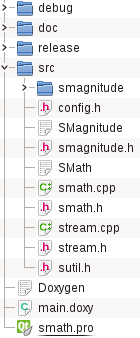
\includegraphics[width=0.25\textwidth]{image/standards-cpp-project-struct}
    \caption[ساختار مورد نیاز برای ایجاد مستند تکنیکی در پروژه‌های \lr{C/C++}]
    {
      
    }
    \label{standards-cpp-struction}
\end{figure}

برنامه‌های زبان برنامه سازی \lr{C/C++} را می‌توان با استفاده از روش‌های متفاوتی
ترجمه کرد. یک روش ترجمه زمانی است که پروژه به صورت کامل تست شده و آماده فاز
تحویل پروژه‌ است. در این فاز با استفاده از برنامه‌های بهینه ساز یک ترجمه بهینه
از پروژه ایجاد می‌شود که به مراتب سریع‌تر از حالت عادی پروژه است. از این رو یک
پوشه به نام  \lr{release} در پروژه ایجاد شده و همواره نتیجه ترجمه نهایی پروژه در
آن ایجاد می‌شود.

ترجمه دیگری که در طی فرآیند توسعه سیستم مورد استفاده قرار می‌گیرد، حالت اشکال
زدا است. در این حالت کدهای اضافه به صورت خودکار به پروزه اضافه شده تا برای دنبال
کردن خط به خط پروژه مناسب باشد. نتایج به دست آمده از این ترجمه نیز در مسیری به
نام \lr{debug} ایجاد می شود.

در نهایت می‌توان با استفاده از ابزارهای مناسب و بر اساس این ساختار، به صورت
خودکار محصول نهایی همراه با مستند تکنیکی را ایحاد کرد. اما پیش از هر چیز نیاز
است که فهرست کاملی از پرونده‌های سرآیند و برنامه‌های نوشته شده ایجاد شود تا
ابزارها بتوانند سرآیندها و برنامه‌های مورد نیاز برای نصب را تعیین کنند. برای
تعیین این پرونده‌ها یک پرونده به نام \lr{<project name>.pro} ایجاد می شود و در
آن فهرست کامل پرونده‌ها ایجاد می‌شود.

\begin{note}
نام این پرونده باید هم نام با پروژه باشد. به یاد داشته باشید که پروژه باید به
صورت کامل در یک پوشه به نام پروژه ایجاد شده باشد، برای نمونه در شکل
\ref{standards-cpp-struction} نه تنها نام پرونده \lr{*.pro} بلکه نام پوشه اصلی
پروژه، هم نام با خود پروژه است.
\end{note}

نام تمام پرونده‌ها با استفاده از کلمه کلید \lr{HEADERS} تعیین می‌شود، در حالت
کلی تعیین پرونده‌های سرآیند به صورت زیر است:

\begin{latin}
\lstset{language=C++}  
\begin{lstlisting}[frame=single] 
HEADERS += <header name> \ 
	... \
	<header name>
\end{lstlisting}
\end{latin}

پرونده‌های پیاده سازی نیز با استفاده از کلمه کلیدی \lr{SOURSES} تعیین می‌شوند.
در حالت کلی این فهرست به صورت زیر ایجاد خواهد شد.

\begin{latin}
\lstset{language=C++}  
\begin{lstlisting}[frame=single] 
SOURCES += <source name> \ 
	... \
	<source name>
\end{lstlisting}
\end{latin}

گاهی ممکن است که پرونده‌های سرآیند و کدهای ایجاد شده تنها برای یک سیستم‌عامل خاص
باشد، در این صورت باید به صورت کامل و تفکیک شده تعیین شوند. در نمونه زیر بر اساس
سکویهای متفاوت کدها و پرونده‌های سرآیند تفکیک شده اند:

\begin{latin}
\lstset{language=C++}  
\begin{lstlisting}[frame=single] 
HEADERS += src/test.h

CONFIG(win) { 
    SOURCES += src/test/win_imp1.cpp \
	src/test/win_imp2.cpp
}
CONFIG(unix) { 
    SOURCES += src/test/unix_imp1.cpp \
	src/test/unix_imp2.cpp
}
\end{lstlisting}
\end{latin}

در این نمونه فرض شده است که برای پرونده سرآیند \lr{test.h} دو نوع پیاده سازی
برای سیستم‌عاملهای یونیکس و ویندوز وجود دارد. از این رو در هر سکو باید
پرونده‌های مناسب ان در محصول نهایی قرار گیرد.
    

\subsection{ساختار پرونده \lr{*.h}}
در یک پرونده سرآیند معمولا تعاریف کلاس‌ها، متدها، توابع و ... آورده می‌شود و
علاوه بر این‌ها باید مستندات این موجودیت‌ها نیز در پرونده‌های سرآیند آورده شود.
ساختاری که برای محل مستندات و تعریف موجودیت‌ها در یک پرونده سرآیند پیشنهاد
می‌شود در قطعه کد \ref{standars-cpp-headers} مشاهده می‌شود.
\begin{latin}
\lstset{language=C++}  
\begin{lstlisting}[frame=single] 
   /*
   *	<License> 
   */
   /**
   *	\file <filenamge>
   *	\date <date>
   *	\brief <a briet documantation about file>
   *	\author <author name>
   *	detailed codumentation about file.
   */
\end{lstlisting}
\label{standars-cpp-headers}
\end{latin}
در ابتدای هر پرونده سرآیند\LTRfootnote{header file} پیمان‌نامه نوشته می‌شود.
نکته اینکه پیمان نامه تنها مستندی است که در مورد پیاده‌سازی است ولی در
سرآیندها هم می‌آید (بنابراین برخلاف سایر مستندات فنی که همگی با \lr{/**}) شروع
می شوند با \lr{/*} شروع می‌شود. پس از پیمان‌نامه مستنداتی در مورد خود پرونده سر‌آیند آورده
می‌شود. مواردی که در این قسمت آورده می‌شود آورده می‌شود عبارتند از:
نام پرونده، تاریخ، نویسنده پرونده،  خلاصه‌ای در مورد پرونده و مستندی در مورد
پرونده به صورت مشروح.

در یک پرونده سرآیند موجودیت‌های مختلفی وجود دارد از جمله تعریف کلاس، متدها و
توابع و غیره. برای تمام این موارد طبق آنچه قبلا گفته شده است باید مستندنویسی
انجام شود. به این ترتیب پس از پیمان‌نامه و مستندات خود پرونده، تعاریف و مستندات
موجودیت‌های مختلف، دیگر محتویات پرونده‌های سرآیند را تشکیل می‌دهند.

\subsection{ساختار پرونده \lr{*.cpp}}
یک پرونده \lr{.cpp} حاوی پیاده‌سازی قسمت‌هایی از پروژه است. مستندات پیاده‌سازی
هر قسمت نیز باید در این پرونده گنجانده شود. همانطور که قبلا هم گفته شد خود
مستندات پیاده‌سازی محل و ساختار خاصی ندارند. اما قالبی برای آن‌ها پیشنهاد می‌شود
که در ادامه شرح داده می‌شود.

 در ابتدای هر پرونده \lr{.cpp} یا \lr{.c} پیمان‌نامه نوشته می‌شود. گاهی ممکن است
 پیمان‌نامه
پرونده‌های سرآیند با پرونده‌هایی که آن سرآیند را پیاده‌سازی می‌کنند متفاوت باشد.
در صورتی که تفاوتی نداشتند می‌توان همان پیمان‌نامه‌ای که در پرونده‌های سرآیند
نوشته می‌شوند را در اینجا نیز قرار داد. مثلا فرض کنید یک گروه نرم‌افزاری یک
مجموعه از سرآیندها را طراحی کرده باشد و پیمان‌نامه خاصی برای آن در نظر گرفته
باشد. سپس گروه‌های دیگری این سرآیندها را پیاده‌سازی کنند. در این مواقع ممکن است
پیمان‌نامه‌ای که گروه‌های پیاده‌ساز به کار می‌برند با پیمان‌نامه گروه طراح
پرونده‌های سرآیند فرق داشته باشد.

پس از پیمان‌نامه مستنداتی در مورد خود پرونده می‌آید. مطالبی از قبیل نام پرونده،
تاریخ، خلاصه‌ای در مورد پرونده و مستندی در مورد پرونده به صورت مشروح (در واقع
همان مواردی که برای پرونده‌های سرآیند نیز مطرح بود). توجه شود که این بخش از
مستند در واقع از نوع مستندات فنی است ولی با این حال در مستندات پرونده‌های حاوی
مستندات پیاده‌سازی آورده می‌شود. سایر مستندات پیاده‌سازی نیز همان مستنداتی است
که برای موجودیت‌های مختلف  پیاده‌سازی شده یا در مورد قطعاتی از برنامه، در
لابه‌لای کدها نوشته می‌شود.


%
% حق نشر 1390-1402 دانش پژوهان ققنوس
% حقوق این اثر محفوظ است.
% 
% استفاده مجدد از متن و یا نتایج این اثر در هر شکل غیر قانونی است مگر اینکه متن حق
% نشر بالا در ابتدای تمامی مستندهای و یا برنامه‌های به دست آمده از این اثر
% بازنویسی شود. این کار باید برای تمامی مستندها، متنهای تبلیغاتی برنامه‌های
% کاربردی و سایر مواردی که از این اثر به دست می‌آید مندرج شده و در قسمت تقدیر از
% صاحب این اثر نام برده شود.
% 
% نام گروه دانش پژوهان ققنوس ممکن است در محصولات دست آمده شده از این اثر درج
% نشود که در این حالت با مطالبی که در بالا اورده شده در تضاد نیست. برای اطلاع
% بیشتر در مورد حق نشر آدرس زیر مراجعه کنید:
% 
% http://dpq.co.ir/licence
%
\chapter{خودکار سازی}

ایجاد پروژه آخرین کاری است که در یک پروژه نرم‌افزاری انجام می‌شود. در این  فاز
تمام برنامه‌های نوشته شده توسط توسعه دهندگان سیستم ترجمه شده و یک برنامه اجرایی
ایجاد می‌شود. کارهایی که در این فاز از پروژه انجام می‌شوند عبارت‌اند از:

\begin{itemize}
  \item ترجمه برنامه‌ها به برنامه‌های اجرایی
  \item ایجاد بسته‌های نرم‌افزاری مبتنی بر برنامه‌های اجرایی
  \item ارزیابی و بررسی کیفیت محصول
  \item ایجاد قابلیت انتقال به روی سیستم‌های متفاوت
  \item ایجاد مستند و راهنما
\end{itemize}

گرچه ممکن است که فرآیند ساخت از یک پروژه به پروژه دیگر متفاوت باشد اما این
فرآیند به صورت مشابه و یکنواخت در تمام آنها اجرا می‌شود. برای نمونه گرچه در
پروژه‌های که از زبانهای مفسری مانند \lr{PHP} استفاده شده باشد ترجمه برنامه به
برنامه‌های اجرایی هرگز انجام نمی‌شود اما مراحل دیگر ساخت پروژه همچنان پا برجا
خواهد بود.

از آنجا که این کار تنها توسط توسعه دهندگان سیستم قابل اجرا و در تمام
پروژه‌ها مورد نیاز است، دور از تصور نیست که این فرآیند به صورت خودکار و توسط یک
ماشین قابل اجرا باشد. خودکار سازی در اینجا نیز به این نکته اشاره دارد. با
استفاده از روش‌های خودکار ساخت پروژه نه تنها می‌توان از میزان هزینه‌ها مانند
زمان و نیروی انسانی کاست بلکه می‌توان به کیفیت کار انجام شده نیز افزود.

ساخت خودکار یک پروژه نرم‌افزاری عبارت است از یک نپشته\LTRfootnote{Script}،
برنامه و یا هر سیستم دیگری که مراحل ساخت یک پروژه را به صورت خودکار و بدون دخالت
کاربر انجام دهد.
    
% History

ابتدایی ترین تلاش‌ها برای خودکار سازی فرآیند ساخت توسط توسعه دهندگان سیستم‌ها
بود. توسعه دهندگان با استفاده از برنامه‌ها و نپشته‌ها مترجم‌ها و پیوندگرها را با
استفاده از دستورهای خط فرمان فراخوانی و با استفاده از آن برنامه‌های
اجرایی را ایجاد می‌کردند. برای نمونه با استفاده از نپشته زیر که در سکوی لینوکس
قابل اجرا است می‌توان تمام پرونده‌های ایجاد شده در یک پروژه سی را ترجمه کرده و
یک برنامه اجرایی ایجاد کرد.

\begin{latin}
\lstset{language=BASH}  
\begin{lstlisting}[frame=single] 
#!/bin/bash
DIR="$1"
OUT="$2"
[ "$DIR" == "" ] && DIR="."
fileArray=($(find -name "*.c"))

#Compile and creat object file
for file in ${fileArray[*]}
do
	g++ -Wall -O $file -o ${file}.o
done

#Link all objrct file
for file in ${fileArray[*]}
do
	g++ ${file}.o $OUT
done

\end{lstlisting}
\end{latin}

با استفاده از این نپشته تمام پرونده‌های \lr{*.c} در یک مسیر با استفاده از مترجم
\lr{g++} ترجمه شده و با استفاده از پیوندگر\LTRfootnote{Linker} یک برنامه اجرای
ایجاد می‌شود.
گرچه این نپشته بسیار ساده است اما به عنوان ابتدایی ترین سیستم‌های خودکارسازی
فرآیند ساخت مورد استفاده قرار می‌گرفته است.

استفاده از دستورهای خط فرمان و ترجمه تک تک برنامه‌های نوشته شده و درنهایت ایجاد
یک برنامه اجرایی با استفاده از یک پیوندگر ساده است. اما زمانی که نیاز به ترجمه
پروژه‌های بزرگ که از قطعه‌های متفاوتی ایجاد شده‌اند و بین آنها وابستگی از پیش
تعریف شده‌ای وجود دارد استفاده از این روش‌های ساده مناسب نیست.

تلاش بعدی توسعه دهندگان سیستم‌های نرم‌افزاری منجر به ایجاد برنامه‌ها و زبانهای
جدید برای خودکار سازی فرآیند ساخت شد. از این میان می‌توان به زبان \lr{Make}
اشاره کرد. این زبان خودکار سازی را می‌توان به عنوان یک جایگزین مناسب برای
نپشته‌های ابتدایی در نظر گرفت. نپشته‌های مورد استفاده در این ابزار امکان نوشتن
وظایف متفاوت مانند ترجمه و پیوند به صورت متوالی  وجود دارد. نسخه‌های ایجاد شده
توسط گروه \lr{GNU} نه تنها توانایی یاد شده را فراهم کرده است بلکه توانایی ساخت
موازی، توزیع شده و یا ایجاد بر اساس وابستگی‌ها نیز فراهم شده است.

اما این تنها آغاز راه بود و فرآیند ساخت به سرعت پیچیده شد. در ابتدا فرآیند ساخت
تنها به ترجمه و پیوند برنامه‌ها توجه داشت. امروزه فرآیند ساخت انقدر پیچده شده
است که نه تنها مترجم‌ و پیوندگرها مورد استفاده قرار می‌گیرد بلکه از سیستم‌های
متفاوت دیگر مانند مستندگر، کنترل نسخه، برنامه‌های ارزیابی و بسیاری دیگر مورد
استفاده قرار می‌گیرد. 

در حال حاضر فرآیند ایجاد شامل وظایف متفاوتی چه قبل از ترجمه و چه بعد از ترجمه
می‌شود. فرآيند ساخت آن چنان پیشرفت کرده است که امروزه بر فرآیند توسعه سیستم‌های
نرم‌افزاری تاثیر گذاشته و منجر به ایجاد متدلوژی‌های جدیدی شده است.

% TODO : maso 1391 : روش‌های CI و ایجاد توزیع شده را باید بررسی کنم

% New breed of solutions

امروزه گونه‌های جدید ابزارهای خودکار سازی فرآیند ساخت امکانات بسیار متفاوت و
مناسبی را ارائه می‌کنند.
این ابزارها به صورت‌های متفاوتی چون نرم‌افزارهای متن باز و یا تجاری ارائه
می‌شوند.
در بسیاری از این ابزارها تمرکز به روی اجرای نپشته‌های ایجادگر است در حالی که
گونه‌های دیگر با توجه به کارهای مورد نیاز پیش و پس از فرآیند ساخت تلاش دارند که
ابزارهای مناسب برای ساده سازی این فرآیند را ارائه کنند. هدف اصلی در ساده سازی
فرآیند ساخت فراخوانی راحت مترجم‌ها، پیونگرهای و دیگر ابزارهای مورد نیاز در
فرآیند ساخت است.
استفاده از این ابزارها در فرآیندهای توسعه مبتنی بر ساخت\LTRfootnote{Continous
Integeration} بسیار اساسی است تا جایی که توسعه سیستم بدون این سیستم‌ها غیر ممکن
می شود.


% Advanced build automation

ابزارهای مدرن ساخت از پیشکارهای\LTRfootnote{Agent} دور برای ایجاد پروژه به صورت
توزیع شده استفاده می‌کنند. واژه ساخت توزیع شده\LTRfootnote{Distributed
builds} به معنی فراخوانی مترجم و پیوندگر به صورت توزیع شده به روی ماشین‌های
متفاوت است که منجر به افزایش سرعت فرآیند ساخت می‌شود.
این واژه به صورت معمول با واژه محاسبات توزیع شد\LTRfootnote{Distributed
Processing} به اشتباه گرفته می‌شود.

% Distributed processing means that each step in a process or workflow can be sent
% to a different machine for execution. For example, a post step to the build may
% require the execution of multiple test scripts on multiple machines. Distributed
% processing can send the different test scripts to different machines.
% Distributed processing is not distributed builds. Distributed processing cannot
% take a make, ant or maven script, break it up and send it to different machines
% for compiling and linking.
% 
% The distributed build process must have the machine intelligence to understand
% the source code dependencies in order to send the different compile and link
% steps to different machines. A build automation solution must be able to manage
% these dependencies in order to perform distributed builds. Some build tools can
% discover these relationships programmatically (Rational ClearMake
% distributed[1], Electric Cloud ElectricAccelerator[2]), while others depend on
% user-configured dependencies (Platform LSF lsmake[3])
% 
% Build automation that can sort out source code dependency relationships can also
% be configured to run the compile and link activities in a parallelized mode.
% This means that the compiler and linkers can be called in multi-threaded mode
% using a machine that is configured with more than one core.
% 
% Not all build automation tools can perform distributed builds. Most only provide
% distributed processing support. In addition, most solutions that do support
% distributed builds can only handle C or C++. Build automation solutions that
% support distributed processing are often make based and many do not support
% Maven or Ant.
% 
% An example of a distributed build solution is Xoreax's IncrediBuild[4] for the
% Microsoft Visual Studio platform or the open-source CMake[5]. These may require
% particular configurations of a product environment so that it can run
% successfully on a distributed platform—library locations, environment variables,
% and so forth.

از سویی استفاده از پیشکارهای متفاوت با گونه‌های متفاوت امکان ایجاد یک سیستم
نرم‌افزاری مبتنی بر سکو‌های متفاوت را نیز امکان پذیر می‌سازد. پیشکارهایی که به
روی سکوی لینوکس\LTRfootnote{Linux} تعبیه شده‌اند سیستم نرم‌افزاری را برای این
سکو ترجمه و به برنامه اجرای تبدیل می‌کنند در حالی که پیشکارهای تعبیه شده به روی
سکوی ویندوز\LTRfootnote{Windows} کار مشابه‌ای را برای سیستم عامل ویندوز انجام
می‌دهند.

% Advantages

خودکارسازی فرآیند ایجاد، منافع زیادی برای گروه توسعه به دنبال دارد. به عنوان
نمونه برخی از این موارد عبارت‌اند از:

\begin{itemize}
  \item افزایش کیفیت محصولها
  \item تسریع در فرآیند ایجاد
  \item کاهش کارهای بیهوده
  \item کاهش اشتباه در فرآیند ساخت
  \item کاهش وابستگی به فرد
  \item نگهداری تاریحچه ساخت برای دنبال کرده ایرادها
  \item کاهش هزینه‌ها
\end{itemize}

% Types
%     On-Demand automation such as a user running a script at the command line
%     Scheduled automation such as a continuous integration server running a nightly build
%     Triggered automation such as a continuous integration server running a build on every commit to a version control system.
% Requirements of a build system
% 
% Basic requirements:
% 
%     Frequent or overnight builds to catch problems early.[7][8][9]
%     Support for Source Code Dependency Management
%     Incremental build processing
%     Reporting that traces source to binary matching
%     Build acceleration
%     Extraction and reporting on build compile and link usage
% 
% Optional requirements:[10]
% 
%     Generate release notes and other documentation such as help pages
%     Build status reporting
%     Test pass or fail reporting
%     Summary of the features added/modified/deleted with each new build

در تمام فرآیندهای ساخت ایجاد مستند تکنیکی و کاربری یکی از مراحل ایجاد بوده و
بدون آن فرآیند ایجاد نرم‌افزار ناقض خواهد بود. در این گفتار ابزارهای خودکار سازی
فرآیند ساخت معرفی شده و تنظیم‌های مورد نیاز برای ایجاد مستند تکنیکی در آنها
تشریج می‌شود.

نکته‌ای که باید در این گفتار به آن توجه داشت این است که، همواره فرض بر این است
که در فرآیند توسعه از استانداردهای تعریف شده در این کتاب استفاده شده است. در غیر
این صورت مراحل و تنظیم‌های مورد نیاز کمی متفاوت خواهد بود.




\section{مدیریت بسته کلاه قرمز}


% در این قسمت باید در مورد این سیستم مدیریت بسته به صورت کامل بحث شود
\lr{RPM} یا مدیریت بسته کلاه قرمز\LTRfootnote{\Gls{red hat package manager}} یک
مجموعه ابزار نرم‌افزاری برای ایجاد و نصب و راه اندازی سیستم‌های نرم‌افزاری است. می‌توان
گفت که پیشینه \lr{RPM} به صورت جدایی ناپذیری با پیشینه سیستم عامل لینوکس در هم
آمیخته است، از این رو بررسی پیشینه‌ لینوکس مفید است. لینوکس یک پیاده سازی کامل
از سیستم‌های عمل شبیه \lr{Unix} است که مانند یک طوفان دنیای محاسبات رایانه‌ای را
درنبردید.

هم زمان با توسعه و گسترش یافتن لینوکس، رایانه‌های شخصی تولید شده مبتنی بر
فن‌آوری \lr{Intel}، که تا پیش از آن اسیر سیستم ترسناک و سیری ناپذیر ویندوز بوند،
به رایانه‌های کاملا چندکاره\LTRfootnote{Fully Multitasking}، با قابلیت استفاده
از شبکه و ایستگاهای کاری شخصی تبدیل شدند. تمام این تعییرها در سخت‌افزارها و
رایانه‌ها به دلیل زمان زیاد مورد استفاده در پردازشها و نیاز شدید استفاده از شبکه
بود.

برای به کار بردن بسیاری از سخت افزارها، شرکت‌های تولید کنند لوح‌های فشرده حاوی
سیستم‌عامل لینوکس و نرم افزارهای مورد نیاز آن را روانه بازار می‌کنند در حالی که
بسیاری از این نرم‌افزارها در شبکه جهانی قابل دسترس هستند.
سرهم بندی کردن نرم‌افزارهای مورد نیاز در سیستم‌عامل لینوکس بر اساس توزیع مورد
استفاده آن متفاوت است اما انچه که مهم است این است که عبارت \'پول هرچه را بدهی
آن را داری\' در اینجا دیگر صادق نیست.

یکی از توزیع‌های لینوکس که نام منحصر به فرد لینوکس کلاه قرمز\LTRfootnote{Red
Hat Linux} را یدک می‌کشید که توسط یک شرکت هم نام با آن توسعه می‌یافت. این توزیع
از سیستم‌عامل لینوکس کمی با دیگر توزیع‌های لینوکس موجود متفاوت بود. یکی از
مشکل‌ترین کارهای کاربران لینوکس تعیین این بود که کدام قسمت از نرم‌افزارهای موجود
در یک توزیع خاص از این سیستم‌عامل باید نصب و مورد استفاده قرار گیرد. در بسیاری
از توزیع‌های لینوکس انتخاب نرم‌افزارهای مورد نیاز برای نصب با استفاده از منوهایی
انجام می‌شد که استفاده از آن بسیار راحت بود و لینوکس کلاه قرمز نیز از این قاعده
مستثنا نبود.

اما تفاوت اصلی این توزیع با دیگر توزیع‌های لینوکس در این بود که سازندگان آن تلاش
داشتند که کاربران برای نصب یک بسته و یا نرم‌افزار کاری بیشتر از انتخاب بسته و یا
نرم‌افزار را انجام ندهند. با این وجود سیستم‌های تجاری یونیکس از سیستمی مشابه با
این نیاز استفاه می‌کرند که سیستم مدیریت بسته\LTRfootnote{Package Manger} نام
داشت. در همین راستا بسیاری از گروها در توزیع‌های متفاوت لینوکس تلاش کردند که
سیستم‌های مشابه‌ای را برای مدیریت بسته‌ها و نرم‌افزارهای ارائه دهند که هیچ کدام
به گستردگی \lr{RPM} نبود.

با گذر زمان توزیع کلاه قرمز لینوکس محبوب‌ترین توزیع لینوکس شد که امروز در دسترس
بسیاری از کاربران است. مهم‌ترین عامل موفقیت این توزیع از سیستم‌عامل لینوکس را
می‌توان \lr{RPM} معرفی کرد. گرچه در اینجا یک توصیف کوتا از این سیستم مدیریت بسته
اورده شده است اما با این وجود می‌توان کاربرد فوق تصور این روش در مدیریت
نرم‌افزارها را به سادگی حس کرد.

اما در دنیای نرم‌افزارهای رایگان یک اصل اولیه وجود دارد که عبارت است: زمانی که
یک سیستم نرم‌افزاری رایگان راهکار مناسب‌تری را ارائه می‌دهد، از آن استفاده کن.
سیستم مدیریتی \lr{RPM} نیز از این قائده مستثنا نیست. از این رو توانایی‌های
موجود در این سیستم به سرعت توجه بسیاری از کاربران و توسعه دهندگان نرم‌افزارهای
رایگان را به خود جلب کرد.

در حال حاضر علاوه بر گروه‌هایی که نرم‌افزارهای رایگان  را توسعه می‌دهند، بسیاری
از شرکت‌ها وجود دارند که محصولات تجاری خود را نیز بر اساس \lr{RPM} روانه بازار
می‌کنند. این شرکت‌ها نه تنها به این نکته دست یافته‌اند که با استفاده از این
سیستم مدیریت نرم‌افزار محصولات آنها راحت‌تر در دسترس مشتریان قرار،
بلکه ایجاد و بسته‌بندی نرم‌افزارها نیز راحت‌تر انجام خواهد گرفت.

% تعیین شود که برای ایجاد باید یک پروند برای توصیف ایجاد کرد.
گرچه هدف از این گفتار تشریح سیستم مدیریت بسته‌ها نیست اما پیش از هر چیر می‌بایست
نکات ابتدایی این سیستم مورد بررسی قرار گیرد. برای ایجاد هر بسته نرم‌افزاری از یک
پرنده استفاده می‌شود که در آن نه تنها پرونده‌های موجود در یک بسته نرم‌افزاری
بلکه روش ایجاد و نصب آنها به صورت کامل توصیف می‌شود. این پرونده یک پرونده متنی
ساده بوده و با پسوند \lr{spec} تعیین می‌شوند. در این پرونده بخش‌های متفاوتی وجود
دارد که مهم‌ترین آنها عبارت اندز از:

\begin{itemize}
  \item \lr{Preamble}
  \item \lr{prep}
  \item \lr{build}
  \item \lr{install}
  \item \lr{file}
\end{itemize}

% ساختار مورد استفاده در این بسته به صورت مقدماتی تشریح شود
\lr{Preamble} خصوصیت‌های کلی بسته مانند نام، نسخه، حق نشر و بسیاری موارد دیگر
تشریح می‌شود در حالی که دیگر قسمت‌ها به توصیف روش نصب و ایجاد پروژه خواهند
پرداخت. ابتدایی ترین بخش در این پرونده قسمت \lr{prep} است که در آن مقدمات ایجاد
نرم‌افزار و بسته بندی آن ایجاد می‌شود. در این بخش کدهای منبع موجود اماده شده و
در مسیرهای مناسب قرار می‌گیرد تا در ادامه فرآیند ترجمه و ایجاد شود. در دو بخش
دیگر که به نام‌های \lr{build} و \lr{install} ایجاد می‌شوند فرآیند ایجاد و نصب
نرم‌افزار ایجاد می‌شود. این دو بخش باید به صورت کاملا مستقل از هم در نظر گرفته
شود چرا که فرآیند نصب به روی رایانه‌های دیگر نیز اجرا می‌شود در حالی که فرآیند
ایجاد تنها به روی ماشینی اجرای می‌شود که بسته نرم‌افزاری در آن ایجاد شده است.

می‌توان گفت که \lr{file} مهم‌ترین قسمت در این پرونده است. در این قسمت تمام
رونده‌های مورد نیاز برای یک بسته و سطح دسترسی به آنها صورت کامل 
تعیین می‌شوند. در این بخش فهرست تمام پرونده‌ها و پوشه‌هایی که باید در بسته ایجاد
شده وجود داشته باشند آورده می‌شود و برای هرکدام تعیین می‌شود که سطح دسترسی
کاربران چیست.

% هدف ما و روش ایجاد این بسته تشریح شود.
مستند فنی یک سیستم نرم‌افزاری نیز بخشی از نرم‌افزار است و باید در فرآیند ایجاد
ایجاد شده و در بسته‌های مناسب قرار گیرد. از این رو باید تنظیم‌های مورد نیاز برای
ایجاد بسته مناسب مستند فنی تعیین شود. در این تنظیم نه تنها روش ایجاد مستند فنی
بلکه نصب آن نیز باید به گونه‌ای تشریح شود که مستند ایجاد شده قابل حمل و نصب به
روی دیگر رایانه‌های نیز باشد. در این میان ممکن است که یک پروژه نرم‌افزاری شامل
زیر پروژه‌های متفاوتی باشد و هر زیر پروژه به صورت مستقل مستند سازی شده باشد.

برای درک بهتر مطالب مطرح شده در این بخش یک پروژه نرم‌افزاری متن باز در نظر
گرفته شده و گام به گام تشریح شده است. این پروژه متن باز که \lr{SMath} نام دارد
یک بسته نرم افزاری است که در محاسبات اعداد بزرگ مورد استفاده قرار
می‌گیرد\cite{smath}. متن برنامه به همراه مستندات این بسته در تارنمای آن قابل
دستیابی است.

\begin{latin}
\lstset{language=TeX}  
\begin{lstlisting}[frame=single] 
http://code.p-simorgh.com/p/SMath
\end{lstlisting}
\end{latin}

این بسته نرم‌افزاری بر اساس قراردادهای تعریف شده در این کتاب ایجاد شده است و
شامل سه زیر پروژه است که عبارت اند از:

\begin{itemize}
  \item \lr{smath}
  \item \lr{smath-test}
  \item \lr{smath-test-suit}
\end{itemize}

زیر پروژه \lr{smath} شامل یک کتابخانه پویا\LTRfootnote{Dynamic Library} است که
محاسبات عددهای بزرگ را پیاده سازی می‌کند در حالی که دو بسته دیگر ارزیابی‌های این
بسته است. زیر پروژه \lr{smath-test} شامل برنامه‌های اجرایی است که در آن از
امکانات این بسته برای محاسبات استفاده شده و زیر پروژه \lr{smath-test-suit}
ارزیابی تمام امکان‌های پیاده سازی شده در این بسته است.

ساختار این پروژه نه انقدر ساده است که برای تشریح تمام موارد مورد نیاز کافی نباشد
و نه انقدر پیچیده که برای آموزش مبانی بسته بندی و خودکار سازی مستند‌های فنی
ناکار آمد باشد.

ایجاد و بسته‌بندی کردن مستند فنی پروژه می‌تواند به دو صورت تصور شود: یک بسته
کاملا مستقل و یا یک زیر بسته. هنگامی که در یک پرونده \lr{spec} روش ساخت و بسته
بندی مستند فنی یک پروژه اورده شود می‌گوییم که بسته به صورت مستقل ایجاد شده است
در حالی که اگر در یک پرونده \lr{spec} علاوه بر ایجاد خود پروژه مستند فنی نیز
ایجاد شود می‌گوییم که مستند فنی به صورت یک زیر بسته ایجاد شده است.

\subsection{یک بسته مستقل}

% اولین کار تعیین خصوصیت‌های کلی است. این خصوصیت‌ها به صورت زیر تعیین می‌شود
نخستین گامل برای ایجاد پرونده \lr{spec} در ایجاد مستند فنی تعیین خصوصیت‌های کلی
بسته مستند فنی است. خصوصیت‌های کلی هر بسته در ابتدای پرونده بسته به صورت جفت‌های
کلید مقدار تعیین می‌شود.  خصوصیت‌های کلی بسته مورد نظر ما به صورت زیر خواهد بود:

\begin{latin}
\lstset{language=TeX}  
\begin{lstlisting}[frame=single] 
Name: smath-doc
Summary: Big integer lib document
Version: 2.0
Release: 0
Group: Development/Documentation
Source: SMath-2.0.0.tar.gz
BuildArch: noarch
\end{lstlisting}
\end{latin}

برای ایجاد تماییز بین بسته‌های نرم‌افزاری و مستند فنی آنها از یک پسوند \lr{doc}
در انتهای نام بسته استفاده می‌شود. در توصیف کوتاهی که برای هر بسته پیش بینی شده
است نیز باید تعیین شود که بسته حاوی مستند فنی است و نسخه بسته نیز باید مشابه با
نسخه بسته نرم‌افزاری ایجاد شده باشد. با این روش می‌توان هموار بسته‌های
نرم‌افزاری و مستندهاای آنها را تمییز داد و تعیین کرد که مستند فنی متعلق به کدام
نسخه از بسته‌های نرم‌افزاری است.

برای جلوگیری از به هم ریختگی بسته‌های ایجاد شده بهتر است که تمام مستندها را نیز
در یک گروه قرار داد. از آنجا که مستند‌های فنی متعلق به توسعه دهندگان سیستم‌های
نرم‌افزاری است، گروه \lr{Development/Documentation} برای این مستندها در نظر
گرفته شده است. این گروه بندی بین توسعه دهندگان سیستم‌های متن باز لینوکس مرسوم
است و هیچ اجباری برای انتخاب آن وجود ندارد.

نکته‌ای که در مورد مستندهای فنی باید در نظر گرفت این است که مستندهای فنی
سیستم‌های نرم‌افزاری به هیچ معماری وابسته نیست مگر این که خود بسته نرم‌افزاری
تنها بر اساس یک معماری خاص ایجاد شده باشد. بر این اساس است که معماری مورد حمایت
در این بسته به صورت 
\lr{noarch}\footnote{واژه \lr{noarch} در اینجه به معنی مستقل از معماری در نظر
گرفته می‌شود که کوتاه شده واژه \lr{No atchitecture} است}
تعیین شده است.
 
% بازگشایی کد و ایجاد پروژه
در گام بعد باید کد منبع آماده شده تا بر اساس آن  بتوان مستند فنی ایجاد شود. از
آنجا که در فرآیندهای ایجاد در سیستم \lr{RPM} همواره یک پرونده فشرده استفاده
می‌شود که در آن کد منبع سیستم نرم‌افزاری به صورت فشرده وجود دارد، کافی است که
پرونده‌ای که شامل کد منبع است را بازگشایی کنیم. همانگونه که در کد بالا قابل
مشاهده است کد منبع مورد استفاده نیز تعیین شده است از این رو فرآیند بازگشایی با
استفاده از دستورهای خط فرمان به صورت زیر انجام خواهد شد:

\begin{latin}
\lstset{language=TeX}  
\begin{lstlisting}[frame=single]
pdir=smath-2.0.0
if [ -d $pdir ]; then
	rm -R -f $pdir
fi
mkdir -p $pdir
cd $pdir
zcat $RPM_SOURCE_DIR/SMath-2.0.0.tar.gz | tar -xvf -
\end{lstlisting}
\end{latin}

در این کد یک پوشه ایجاد شده و کد منبع در آن بازگشایی شده است. استفاده از این
تکنیک زمانی مناسب است که فرآیند ایجاد سیستم‌های نرم‌افزاری متفاوت به صورت همزمان
در حالی اجرا باشد. در این حالت با استفاده از پوشه‌های متفاوت از تداخل‌های
احتمالی میان نرم‌افزارهای جلوگیری می‌شود. اما پیش از هر کاری باید مسیرهای ایجاد
شده را حذف کرد تا تنظیم‌های مورد استفاده در فرآیند قبلی ساخت از بین برود. در
نهایت با بازگشایی متن برنامه در مسیر ایجاد شده می‌توان فرآیند ساخت را ادامه داد.

% ساخت مستند
با ایجاد مسیر مناسب و بازگشایی متن برنامه‌ها شرایط برای ایجاد مستند فنی به صورت
کامل فراهم است. در این مرحله می‌بایست تک تک مستند‌های فنی برای تمام زیر پروژه‌ها
را ایجاد کرد. قطعه برنامه زیر فرآیند ایجاد پروژه را نمایش می‌دهد: 

\begin{latin}
\lstset{language=TeX}  
\begin{lstlisting}[frame=single] 
...
mkdir -p final/doc/
cd smath
doxygen Doxygen
cd ../smath-test
doxygen Doxygen
cd ../smath-test-suit
doxygen Doxygen
\end{lstlisting}
\end{latin}

ابتدایی ترین کاری که باید انجام شود ایجاد مسیر مناسب برای مستند‌های فنی است.
همانگونه که در تعیین استانداردها تعیین شده، تمام مستند‌های فنی باید در مسیر پوشه
\lr{final/doc} ایجاد شوند از این رو پیش از ایجاد مستند فنی زیر پروژه‌ها باید از
وجود این مسیر اطمینان حاصل کرد.

در ادامه این فرآیند با ورود به پوشه هر یک از زیر پروژه‌ها مستند فنی آن ایجاد
می‌شود. مستند فنی با استفاده از دستور خط فرمان \lr{doxygen} و با استفاده
از پرونده‌های پیکره بندی هر پروژه به صورت جداگانه ایجاد می‌شود. 

\begin{note}
همواره فرض بر این است که دستور ایجاد مستند فنی در مسیر هر پروژه به صورت جداگانه
اجرا می‌شود از این رو تعیین مسیر خروجی برای هر زیر پروژه به صورت
\lr{../final/doc} تعیین می‌شود.
\end{note}

در نهایت مستند ایجاد شده باید در مسیرهای مناسب نصب شود. برای این کار کافی است که
مستندهای ایجاد شد در مسیرهای از پیش تعیین شده رو نوشت کرد. در توزیع‌های متفاوت
لینوکس مسیرهای مشخصی برای قرار دادن مستندها در نظر گرفته شده است. مسیر مستندها
در اغلب توزیع‌های لینوکس مشابه است اما گاهی در برخی از نسخه‌های متفاوت است. در
اینجا مسیرهای تعیین شده در توزیع \lr{OpenSUSE} به عنوان مسیر پیش فرض در نظر
گرفته شده و مستندها در این مسیر رونوشت شده است. از این رو برنامه نصب مستند فنی
به صورت زیر خواهد بود:

\begin{latin}
\lstset{language=TeX}  
\begin{lstlisting}[frame=single] 
%install
...
mkdir -p %{buildroot}/usr/share/doc/
cp -R final/doc/ %{buildroot}/usr/share/
\end{lstlisting}
\end{latin}

همانگونه که در این نپشته قابل مشاهده است، فرآیند نصب مستندهای فنی تنها معادل با
رو نوشت کردن مستندهای ایجاد شده در مسیرهای مناسب است. 

در نهایت باید تعیین کرد که چه پرونده‌های در بسته قرار می‌گیرند. در سیستم مدیریت
بسته \lr{RPM} تنظیم‌های پیش‌فرضی برای پرونده‌های مستند در نظر گرفته شده است از
این رو نیازی به تعیین تنظیم خاص در این قسمت نیست و تنها کافی است که فهرست
پرونده‌ها را تعیین کرد. برای نمونه در اینجا پرونده مستندها به صورت زیر در بسته
جای می‌گیرد:

\begin{latin}
\lstset{language=TeX}  
\begin{lstlisting}[frame=single] 
%docdir /usr/share/doc
/usr/share/doc
\end{lstlisting}
\end{latin}

همانگونه که در برنامه قابل مشاهد است، تنها مسیر مستند در فهرست پرونده‌ها
قرار گرفت است. از انجا که تمام مستندهای ایجاد شده همگی در این مسیر نصب (یا رو
نوشت شده است) تنها کافی است که این مسیر به همراه تمام پرونده‌های موجود را در
بسته ایجاد شده قرار داد. در نهایت پرونده \lr{spec} برای مستند فنی این بسته به
صورت زیر خواهد بود:


\begin{latin}
\lstset{language=TeX}  
\begin{lstlisting}[frame=single] 
%define name smath-doc
%define version 2.0
%define release 0

Name: %{name}
Summary: Big integer lib document
Version: %{version}
Release: %{release}
License: GPL
Group: Development/Lib
Vendor: Simorgh 
Packager: Mostafa Barmshory <mostafa.barmshory@p-simorgh.com>
URL: http://code.p-simorgh.com/index.php/p/smath/
Source: SMath-%{version}.%{release}.tar.gz
BuildArch: noarch

%description
It is simple big integer lib. 

%prep
pdir=SMath-%{version}.%{release}
if [ -d $pdir ]; then
	rm -R -f $pdir
fi
mkdir $pdir
cd $pdir
zcat $RPM_SOURCE_DIR/SMath-%{version}.%{release}.tar.gz | tar -xvf -

%build
pdir=SMath-%{version}.%{release}
cd $pdir
mkdir -p final/doc/
cd smath
doxygen Doxygen
cd ../smath-test
doxygen Doxygen
cd ../smath-test-suit
doxygen Doxygen

%install
pdir=SMath-%{version}.%{release}
cd $pdir
mkdir -p %{buildroot}/usr/share/doc/
cp -R final/doc/ %{buildroot}/usr/share/

%files
%docdir /usr/share/doc
/usr/share/doc
\end{lstlisting}
\end{latin}

% نصب 
در نهایت با نصب بسته ایجاد شده مستندهای فنی نرم‌افزار در سیستم نصب شده و قابل
استفاده می‌باشد. ایجاد بسته با استفاده از دستور \lr{rpmbuild} انجام می‌شود.
ایجاد بسته مورد نظر به صورت زیر خواهد بود.

\begin{latin}
\lstset{language=TeX}  
\begin{lstlisting}[frame=single] 
rpmbuild -ba smath2.spec
\end{lstlisting}
\end{latin}

\subsection{زیر بسته}

نمی‌توان مستندهای تکنیکی را مستقل از خود بسته‌های نرم‌افزاری در نظر گرفت از این
رو ایجاد مستندهای فنی نیز می‌تواند توام با ایجاد خود بسته‌های نرم‌افزاری انجام
شود. در این حالت از روش زیر بسته‌ها استفاده می شود.

در این روش یک بسته به عنوان بسته اصلی در نظر گرفته می‌شود و دیگر بسته‌ها به صورت
زیر بسته‌های بسته اصلی در نظر گرفته می‌شود. برای نمونه بسته مستند فنی می‌تواند
به عنوان زیر بسته‌ای از بسته اصلی \lr{smath} در نظر گرفته شود.

سیستم مدیریت بسته \lr{RPM} راهکارهای مناسبی را برای ایجاد و مدیریت بسته‌ها و زیر
بسته‌ها ایجاد کرده است. در اینجا نیز برای هر زیر بسته دسته‌ای از اطلاعات کلی
وجود دارد که به صورت زوج‌های مقدار کلید تعریف می‌شوند با این تفاوت که اطلاعات
کلی هر زیر بسته با استفاده از برچسب \lr{package} تعیین می شود.

تکه برنامه زیر خصوصیت‌های کلی مورد نظر برای بسته مستند فنی را تعیین کرده است:

\begin{latin}
\lstset{language=TeX}  
\begin{lstlisting}[frame=single] 
%package doc
Summary: Big integer lib document.
Group: Development/Documentation
BuildArch: noarch
%description doc
It is simple big integer lib. Documentation is used for developer
\end{lstlisting}
\end{latin}

نام هر زیر بسته که بعد از برچسب \lr{package} اورده می‌شود به عنوان یک پسوند از
عنوان بسته اصلی در نظر گرفته می‌شود از این رو نام بسته مستند فنی در اینجا نیز
به صورت \lr{smath-doc} خواهد بود.

تمام خصوصیت‌های تعریف شده برای بسته اصلی در زیر بسته‌ها نیز به ارث می‌رسد و در
صورت نیاز می‌توان آنها را باز نویسی کرد. در اینجا نیز نسخه و بسیار از خصوصیت‌های
دیگر با بسته اصلی یکی است از این رو نیازی به تعیین این خصوصیت‌ها نیست. 

گرچه تمام خصوصیت‌های بسته اصلی توسط زیر بسته‌ها نیز به ارث می‌رسد اما برای هر
زیر بسته می‌بایست خصوصیت‌هایی مانند گروه، و توصیف بسته را باز نویسی کرد. از انجا
که بسته ایجاد شده یک بسته شامل مستندهای فنی است نه تنها توصیف‌های این زیر بسته
باید بیانگر این مطلب باشد بلکه گروه بسته نیز باید به صورت مناسب تعیین شود. از
این رو گروه این زیر بسته به صورت \lr{Development/Documentation} در نظر گرفته شده
است. علاوه بر این ممکن است که بسته اصلی بر اساس معماری خاصی ایجاد شود در حالی که
مستند فنی سیستم به هیچ معماری وابسته نیست. برای تعیین این نکته خصوصیت معماری
مورد استفاده نیز به صورت زیر بازنویسی شده است:

\begin{latin}
\lstset{language=TeX}  
\begin{lstlisting}
BuildArch: noarch
\end{lstlisting}
\end{latin}

گرچه هر زیر بسته می‌تواند از خصوصیت‌های منحصر به فرد خود استفاده کنند اما کدهای
منبع مورد استفاده میان تمام انها مشترک است. بدیهی است  فرآیند آماده سازی کدهای
منبع نیز در تمام زیر بسته‌ها نیز مشترک باشد. زیر بسته مستند فنی نیز از این قائد
مستثنی نیست و مبتنی بر کد منبع کل سیستم ایجاد خواهد شد.

\begin{note}
فرآیند ایجاد کد منبع مشابه به حالی است که در آن از زیر بسته‌ها استفاده نمی‌شود
از این رو در اینجا به آن پرداخته نشده است.
\end{note}

برخلاف اماده سازی کد منبع سیستم، فرآیند ایجاد آن بسیار پیچیده خواهد بود. در این
فرایند نه تنها باید برنامه‌های ایجاد شده به صورت کامل ترجمه، ارزیابی و پیونده
زده شوند، بلکه باید مستندهای فنی و سایر موارد مورد لزوم دیگر نیز ایجاد شود.

ایجاد دیگر بخش‌های پروژه در اهداف این کتاب نمی‌گنجد از این رو تنها روش ایجاد
مستند فنی سیستم مورد نظر است. ایجاد مستند فنی نیز بر اساس روشهای مطرح شده در
بخش قبل خواهد بود. کد مورد نیاز برای ایجاد مستند فنی به صورت زیر خواهد بود.

\begin{latin}
\lstset{language=TeX}  
\begin{lstlisting}[frame=single] 
%build
...
mkdir -p final/doc/
cd smath
doxygen Doxygen
cd ../smath-test
doxygen Doxygen
cd ../smath-test-suit
doxygen Doxygen
\end{lstlisting}
\end{latin}

برخلاف آماده سازی و ایجاد پروژه، که در تمام زیر پروژه‌ها مشترک است، فرآیند نصب
برای هر زیر بسته به صورت مستقل اجرا می‌شود. دور از انتظار نیست که فرآیند نصب
بسته مستند فنی با نمونه‌ای که مستند فنی به صورت مستقل ایجاد می‌شود تفاوتی نداشته
باشد. گرچه فرآیند نصب مستند فنی به صورت مستقل و در بخشی جداگانه ایجاد می‌شود اما
در اینجا نیز مستندهای ایجاد شده تنها در مسیرهای مناسب رو نوشت خواهد شد. فرآیند
نصب بسته مستند فنی نیز به صورت زیر خواهد بود.

\begin{latin}
\lstset{language=TeX}  
\begin{lstlisting}[frame=single] 
%install doc
...
mkdir -p %{buildroot}/usr/share/doc/
cp -R final/doc/ %{buildroot}/usr/share/
\end{lstlisting}
\end{latin}

بخش دیگری که برای هر بسته به صورت مستقل ایجاد می‌شود فهرست پرونده‌های موجود در
هر زیر بسته است. از آنجا که هر زیر بسته ممکن است بر اساس طبیعت خود فهرست متفاوتی
از پرونده‌های پروژه را داشته باشد، مستند فنی نیز شامل تمام پرونده‌های ایجاد شده
در فرآیند مستند سازی خواهد بود. کد زیر تعیین فهرست مستند فنی برای زیر بسته مستند
فنی را نمایش می‌دهد.

\begin{latin}
\lstset{language=TeX}  
\begin{lstlisting}[frame=single] 
%files doc
%docdir /usr/share/doc
/usr/share/doc
\end{lstlisting}
\end{latin}

در نهایت با فراخوانی دستور \lr{rpmbuild} نه تنها تمام بسته‌های نرم‌افزاری بلکه
بسته مستند فنی نیز ایجاد می‌شود. این بسته وابسته به هیچ معماری نبوده و به سادگی
به روی سیستم‌های متفاوت نصب خواهد شد.




% TODO: maos 1391: استفاده از یک بسته نرم‌افزاری دیگر
% از بسته‌های نرم‌افزاری برای توصیف فرآیند استفاده شده است. با استفاده از بسته‌های
% متفاوت می‌توان محصولات خودمان را نیز معرفی کنیم.

\section{\lr{OBS}}

سرویس ساخت \lr{OpenSUSE}\LTRfootnote{Opne Build Service} که با نام اختصاری
\lr{OBS} نمایش دهده می شود یک سکوی توسعه گسترده است. در این سکوی توسعه امکان‌های پایه‌ای مورد
نیاز برای ساخت پروژه‌های متن باز برای سیستم‌عامل‌های لینوکس را فراهم کرده است.
در این سکوی توسعه امکان ایجاد یک سیستم نه تنها بر اساس توزیع‌های متفاوت لینوکس
فراهم شده است بلکه امکان ایجاد بر اساس معماری‌های متفاوت نیز وجود دارد. در حال
حاضر این سرور باز ساخت پروژه‌های متن باز به بیش از 30000 کاربر خدمات داده و بیش
از 160000 بسته را برای معماری‌ها و سیستم‌های عامل متفاوت فراهم کرده
است\cite{buildopensuse}.

% What exactly is the Open Build Service ?

\lr{OBS} در حقیقت محیط توسعه‌ای است که ابزارهای مورد نیاز توسعه دهندگان
پروژه‌های متن باز در فرآیند ایجاد را فراهم کرده است. با استفاده از این ابزار
می‌توان به سادگی پروژه‌های متن باز را نه تنها برای توزیع‌ها متفاوت لینوکس بلکه
برای معماری‌های متفاوت ایجاد کرده و برای استفاده دیگر کاربران آن را به اشتراک
گذاشت.

بزرگترین ایرادی که می‌توان به نرم‌افزارهای توسعه داده شده برای لینوکس وارد کرد،
عدم کاربرد بسته‌های ایجاد شده برای یک توزیع از این سیستم عامل در توزیع‌های دیگر
است. به بیان دیگر زمانی که یک توسعه دهند یک بسته نرم‌افزاری را برای یک توزیع خاص
از لینوکس ایجاد می‌کند (برای نمونه \lr{ReadHat}) در بسیاری از موارد نمی‌توان آن
را برای توزیع‌های دیگر به کار برد.

کارگزار ساخت \lr{OpenSUSE} تنها کارگزار متن بازی است که امکان ایجاد بسته‌های
نرم‌افزاری را در یک زمان برای توزیع‌های متفاوت لینوکس و تمام
ابزارهای مورد نیاز در این فرآیند را به بهترین شکل  فراهم کرده است.

%  With the system imaging tool
% KIWI, open source developers can more quickly build a Linux distribution that
% meets their needs, rigorously test it to ensure product quality, and easily
% package it for quick installation. Users can easily find the latest open source
% packages they are looking for and will be able in the future to build customized
% distributions.
%
% The Open Build Service is completely open source, giving developers and users
% free and full access to build their choice of Linux packages, whether they are
% based on openSUSE, SUSE Linux Enterprise, Fedora, Debian, Ubuntu or other
% projects.

% Can anybody build packages with the Open Build Service ?

برای ایجاد یک پروژه به روی این کارگزار به آدرس آن (\lr{build.opensuse.org})
مراجعه کرده و یک  کاربر ایجاد کنید. با استفاده از این کاربر می‌توان پروزه‌های متن باز را ایجاد کرده و
مبتنی بر آنها مخزن نرم‌افزاری برای توزیع‌های متفاوت لینوکس ایجاد کرد.

این کارگزار ساخت نه تنها با استفاده از واسط تارنما بلکه با استفاده از برنامه‌های
کاربردی متفاوت قابل دسترسی است. در تارنمای این کارگزار فهرست تمام پروژه‌های
موجود بوده و گزارش کاملی از وضعیت جاری کارگزار نمایش داده شده است. در این تارنما
راهنمای کامل کاربری ایجاد شده است که کاربران را در استفاده از آن یاری می‌کند.


%
% But bear in mind that the Open Build Service is a community support project. So
% please, if you plan to build packages, make sure
%
%     your package really adds something new to the community
%     you talk to people that are working on similar packages or topics
%     to rather help on existing packages than duplicating packages
%     you let people know about what you're doing to find other interested community members. Mailinglists are the right place to do that.
%
% Always remember, regardless how much build power is added to the build service,
% it can be eaten up by not so usefull packages ;-)


% Can the Open Build Service build package for other distributions ?

گرچه در هنوز در این کارگزار ساخت، سیستم‌عامل‌هایی مانند مک\LTRfootnote{Mac} و
یا ویندوز حمایت نمی‌شود اما امکان ساخت بسته‌های نرم‌افزاری در قالب‌های
\lr{RPM}\LTRfootnote{Read Hat Package Manager} و \lr{debian} وجود دارد. در این
کارگزار توزیع‌های \lr{Debian}، \lr{Ubuntu}، \lr{Fedora}، \lr{CentOS} و
\lr{Mandriva} به صورت مستقیم مورد حمایت قرار می‌گیرد.


% Can I build my own distribution with the Open Build Service ?
%
% KIWI, used by the Build Service, supports the generation of image files.
% openSUSE 11.2 was produced completely using the Build Service, including images.
% For an example of customising the distribution, look at the KDE:Medias project,
% which offers stable openSUSE updated with the most recent KDE release.

% Why is the Open Build Service unique ?
این کارگزار ساخت یکی از کارگزاران ساخت نرم‌افزاری منحصر به فرد به شمار می‌رود.
برخی از خصوصیت‌های این کارگزار ساخت که آن را به یک نمونه منحصر به فرد تبدیل کرده
است عبارت است از:

\begin{itemize}
  \item می‌یابد این کارگزار کاملا متن باز توسعه.
  \item این کارگزار فرآیند ایجاد بسته‌های نرم‌افزاری را بسیار ساده کرده است.
  \item با استفاده از این کارگزار می‌توان بسته‌ها را به صورت عملی مورد آزمون
  قرار داد.
  \item این روش بهترین رویکرد برای ایجاد مخزن‌های بزرگ نرم‌افزاری است.
  \item با استفاده از آن می‌توان بسته‌های نرم‌افزاری را برای توزیع‌های متفاوت از
  لیونکس ایجاد کرد.
  \item این کارگزار واسط بسیار ساده کاربری برای نصب بسته‌های نرم‌افزاری ایجاد
  کرده است.
  \item یک پارچگی سیستم همواره حفظ می‌شود به این معنی که اگر یک بسته مورد
  استفاده در سیستم تغییر کرد، بسته‌های وابسته به صورت خودکار ترجمه و ایجاد
  می‌شوند.
\end{itemize}

گرچه با استفاده از واسط تارنمای این کارگزار ساخت کاربران به سادگی قادر خواهند
بود فرآیند ایجاد سیستم‌های نرم‌افزاری را مدیریت کنند اما امکان استفاده از خط
فرمان در فرآیند ساخت نیز فراهم شده است. با استفاده از بسته نرم‌افزاری \lr{osc}
که برای بسیاری از توزیع‌های لینوکس موجود است، کاربران قادراند با استفاده از خط
فرمان فرآیند ایجاد سیستم نرم‌افزاری خود را مدیریت کنند.

گرچه تارافزار این کارگزار روشی بسیار ساده برای مدیریت فرآیند ساخت را فراهم کرده
است اما با استفاده از خط فرمان می‌توان فرآیند ساخت را به صورت محلی اجرا کرده و
خطاهای موجود در فرآیند ساخت را شناسایی و رفع کرد. بسته \lr{osc} محیط ساخت
بسته نرم‌افزاری را به روی رایانه نصب کرده و کاربران را قادر می‌سازد که نه تنها
فرآیند ساخت بلکه رفع خطای این فرآیند را به روی رایانه شخصی خود اجرا کنند که یک
روش بسیار مناسب برای آموزش، رفع خطا و بررسی صحیت فرآیند ساخت است.

\subsection{پروژه}

در این کارگزار ساخت معادل با هر کاربر یک پروژه ایجاد می‌شود که هم نام با نام
کاربری است. پروژه در اینجا به معنی یک گردایه از بسته‌های نرم افزاری است که با یک
دیگر یک یا چند مخزن نرم‌افزاری را سازماندهی می‌کنند. برای نمونه فرض کنید که یک
مخزن از بسته‌های نرم‌افزاری مورد استفاده در رمزنگاری موجود است. تمام این
بسته‌های نرم‌افزاری را می‌تواند در قالب یک مخزن نرم‌افزاری در نظر گرفته و به
صورت یک پروژه در این کارگزار مدیریت کرد. در این بخش پروژه به معنی موجودیتی در
نظر گرفته می‌شود که در این کارگزار تعریف شده است و مواردی که هدف تعریف دیگر از
پروژه باشد به آن اشاره خواهد شد.

پروژه اصلی ایجاد شده برای هر کاربر به عنوان پروژه خانه\LTRfootnote{Home Project}
در نظر گرفته می‌شود. این نام گذاری به این دلیل است که کاربران مجار به ایجاد
پروژه‌های دیگر خارج از پروژه اصلی خود نیستند از این رو پروژه اصلی هر کاربر 
پروژه خانه وی در نظر گرفته می‌شود.

در تارافزار این کارگزار گزینه‌های متفاوتی برای مدیریت پروژه‌ها وجود دارد که
امکان خصوصیت‌های متفاوتی از پروژه را فراهم کرده است. مهم‌ترین خصوصیت‌های قابل
تغییر در فهرست زیر آورده شده است.

\begin{itemize}
  \item گزار حالت کلی پروژه
  \item مدیریت بسته‌ها
  \item مدیریت مخزن نرم‌افزاری
  \item مدیریت نیازها
  \item مدیریت کاربران
\end{itemize}

با استفاده از گزارش‌های ایجاد شده می‌توان تعیین کرده که کدام بسته‌های نرم‌افزاری
ترجمه و یا کدام بسته‌ها در فرآیند ایجاد و بسته بندی با مشکل رو برو شده اند و یا
حتی تعیین کرد که بسته‌های مورد نظر برای کدام سیستم‌های عامل ایجاد و یا در حال
ساخت هستند. مدیریت بسته‌های امکان اضافه و مدیریت کردن بسته‌های نرم‌افزاری به
مخزن‌های ایجاد شده را فراهم می‌کند در حالی که مدیریت نیازها و کاربران امکان
تعیین نیازهای جدید در بسته‌ها و یا کاربران مجاز بسته‌های ایجاد شده را فراهم
می‌کند.

معادل با هر مخزن، در سیستم یک مکان در نظر گرفته می‌شود و نتایج به وجود امده از
فرآیند ساخت در آنها قرار گرفته می‌شود. از این رو با استفاده از ابزارهای مدیریت
بسته می‌توان به سادگی بسته‌های نرم‌افزاری را روی رایانه‌های مقصد نصب و به روز
رسانی کرد. از آنجا که هر پروژه نه تنها برای توزیع‌های متفاوت بلکه نسخه‌های
متفاوت ایجاد می‌شود نیاز است که مخزن‌های متفاوتی برای یک پروژه در نظر گرفت. از
این جهت مخزن در اینجا معادل با سکویی در نظر گرفته می‌شود که سیستم برای آن ایجاد
شده است. به این ترتیب در مدیریت مخزن‌ها، سیستم‌های عامل
هدف\LTRfootnote{Distance Machine} تعیین، و بیان می‌شود که بسته‌های ایجاد شده
برای هر سیستم عامل چه رفتاری باید داشته باشد.

در شکل  \ref{image/standard/build/opensuse-project-overview} یک نمایش از واسط
مدیریت پروژه نمایش داده شده است. همانگونه که در این شکل قابل مشاهده است علاوه بر
گزارش کلی فرآیند ساخت سامانه مناسب برای مدیریت پروژه در نظر گرفته شده است.

\begin{figure}
\centering
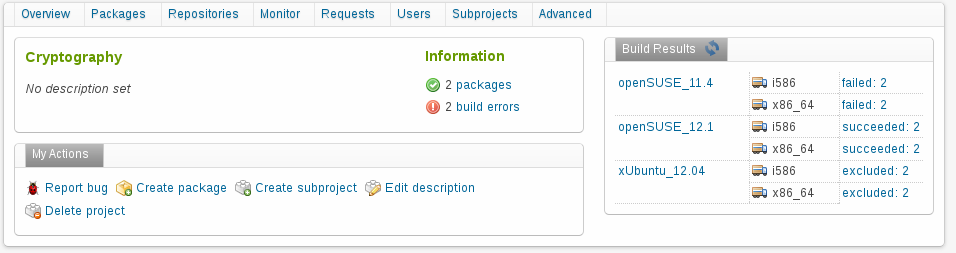
\includegraphics[width=0.75\textwidth]{image/standard/build/opensuse-project-overview.png}
\caption[مدیریت پروژه‌ها در کارگزار ساخت]{
	مدیریت پروژه به قسمت‌های متفاوتی مانند، مخزن‌ها، زیر پروژه‌ها، خصوصیت‌ها و دیگر
	خصوصیت‌های دیگر تشکیل شده است. با استفاده از این سامانه می‌تواند به سادگی
	پروژه‌های ایجاد شده را مدیریت کرد.
}
\label{image/standard/build/opensuse-project-overview}
\end{figure}

به این نکته اشاره شد که هر کاربر نمی‌تواند خارج از پروژه خانه پروژه دیگری داشته
باشد اما به این معنی نیست که کاربر تنها می‌تواند یک پروژه داشته باشد. در این
کارگزار از مفهوم زیرپروژه نیز حمایت می‌شود. هر پروژه می‌تواند از زیر پروژه‌های
متفاوتی ایجاد شده باشد و به همین ترتیب هر زیر پروژه می‌تواند زیرپروژه‌های خاص
خود را داشته باشد. تمام پروژه‌ها و زیر پروژه‌ها به صورت یکسان مدیریت می‌شوند از
نظر کاربردی و امکانات هیچ تفاوتی با یکدیگر ندارد. استفاده از این مفهوم در این
کارگزار تنها برای مدیریت پروژه‌های ایجاد شده بوده و کار برد دیگر ندارد. از این
رو نه تنها کارگزار بلکه کابران می‌توانند تنها با دیدن مسیر هر بسته تعیین کنند که
این بسته به وسیله چه کسی ایجاد شده است.

بر این اساس می‌توان گفت پیش از ایجاد مستند‌های فنی در این کارگزار ساخت می‌بایست
یک فرآیند ابتدایی را برای آماده سازی کارگزار انجام داد. این فرآیند را می‌توان به
صورت مراحل زیر مرتب کرد.

\begin{itemize}
  \item تعیین مخزن‌ها\LTRfootnote{Repository}
  \item اضافه کردن کد برنامه\LTRfootnote{Source code}
  \item تعیین نپشته‌های ایجاد\LTRfootnote{Build Script}
\end{itemize}

همانگونه که اشاره شده هر مخزن معادل با یک سیستم‌عامل است که بسته‌های ایجاد شده
به منظور نصب و راه اندازی به روی آن ایجاد می‌شوند و در نهایت در مسیرهای مناسب
برای همان سیستم‌عامل ساماندهی می‌شوند. از این رو در فرایند تعیین مخزن کافی است
که سیستم‌های عامل مقصد برای پروژه را تعیین کرد. در شکل 
\ref{image/standard/build/opensuse-project-repository}
نمای کلی مدیریت مخزن نمایش داده شده است.

\begin{figure}
\centering
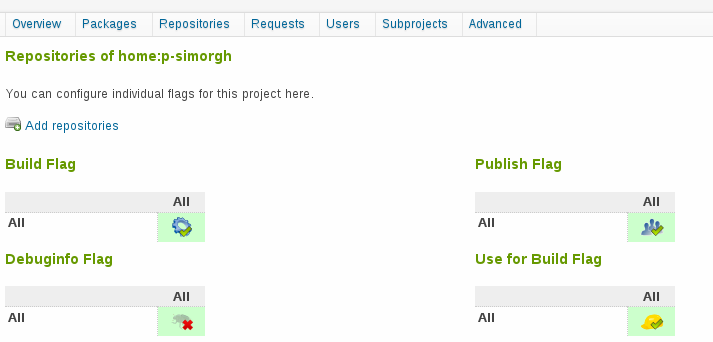
\includegraphics[width=0.75\textwidth]{image/standard/build/opensuse-project-repository.png}
\caption[]{}
\label{image/standard/build/opensuse-project-repository}
\end{figure}

گرچه تولید مستند فنی مستقل از سیستم‌های عامل مورد استفاده است اما در حالت کلی
نمی‌توان با استفاده از کارگزار ساخت بسته‌های مناسب مستند فنی را بدون در نظر
گرفته سکوهای مورد استفاده ایجاد کرد. درحال حاضر سیستم‌عامل‌های متفاوتی در این
کارگزار ساخت مورد حمایت قرار می‌گیرد که در فهرست زیر آورده شده است:

\begin{itemize}
  \item \lr{openSUSE}
  \item \lr{Debian}
  \item \lr{Fedora}
  \item \lr{RedHat}
  \item \lr{CentOS}
  \item \lr{Mandriva}
  \item \lr{Ubuntu}
\end{itemize}

گرچه بسته مستند فنی برای تمام سیستم‌های متفاوت به صورت یکتا ایجاد و تعریف می‌شود
و حتی مستند‌های ایجاد شده به روی هر سیستم‌عامل قابل انتقال به دیگر سیستم‌های
عامل هستند،اما ممکن است فرآیند نصب این بسته‌های در هر سکو متفاوت باشد.
از این رو فرآیند ساخت بسته مستند فنی برای هر سکو متفاوت بوده و از اصول خاص
تعریف شده در سکوی مورد نظر ایجاد می‌شود..

در گام بعد کد منبع بسته نرم افزاری برای کارگزار ساخت تعیین شود. معمولا کد منبع
برای هر سیستم نرم‌افزاری به صورت یک پرونده فشرده به پروژه اضافه می‌شود اما در
برخی موارد از چندین پرونده فشرده برای این منظور استفاده می‌شود.

فرآیند ساخت سیستم‌های نرم‌افزاری در قالب یک بسته نرم‌افزاری در این کارگزار
مدیریت می‌شود. هر بسته نرم‌افزاری شامل تعداد دلخاهی کد منبع است که در کنار
یکدیگر ترجمه شده و سیستم نرم‌افزاری را ایجاد می‌کنند. استفاده از واژه بسته
نرم‌افزاری برای مدیریت یک سیستم نرم‌افزاری و کدهای منبع آن به این معنی نیست که
نتیجه ایجاد یک سیستم نرم‌افزاری تنها می‌تواند به یک بسته منجر شود بلکه در اقلب
موارد نتیجه ساخت سیستم‌های نرم‌افزاری چندی بسته خواهد بود. در ادامه این بخش
منظور از بسته همان مفهومی است که در کارگزار ساخت استفاده می‌شود و در سایر موارد
به آن اشاره خواهد شد.

دور از انتظار نیست که نتیجه ایجاد یک بسته منجر به ایجاد بسته‌های نرم‌افزاری
متفاوتی باشد که یکی از آنها مستند فنی سیستم است. به هر حال در کارگزار ساخت این
حالت پیش بینی شده و امکان ایجاد بسته‌های نرم‌افزاری متفاوت مبتنی بر یک کد منبع
فراهم شده است.

کارگزار ساخت توانایی مدیریت بسته‌های نرم‌افزاری را نیز فراهم کرده است. از این رو
برای هر بسته یک سری ابزار مدیریت فراهم شده است که کاربر با استفاده از آن
می‌تواند به سادگی بسته‌های معرفی شده در سیستم را مدیریت کند. در شکل 
\ref{image/standard/build/opensuse-project-package} ابزارهای موجود برای مدیریت
یک بسته نمایش داده شده است. مهمترین توانایی‌های ایجاد شده برای مدیریت یک بسته در
فهرست زیر آورده شده است:

\begin{itemize}
  \item گزارش حالت کلی بسته
  \item مدیرت کد منبع
  \item مدیریت تقاضا‌ها برای یک بسته
\end{itemize}

در گزارش کلی ایجاد شده برای هر بسته نه تنها تعداد کدهای منبع بلکه تعداد ساخت‌های
موفقیت آمیز، تعداد خطاها، حالت ایجاد بسته برای هر مخزن و سایر موارد دیگر نمایش
داده می‌شود. با استفاده از مدیریت تقاضاها می‌تواند تعیین کرد که نیازهای کاربران
بسته چیست و برای برطرف کردن این نیازها برنامه ریزی کرد.

\begin{figure}
\centering
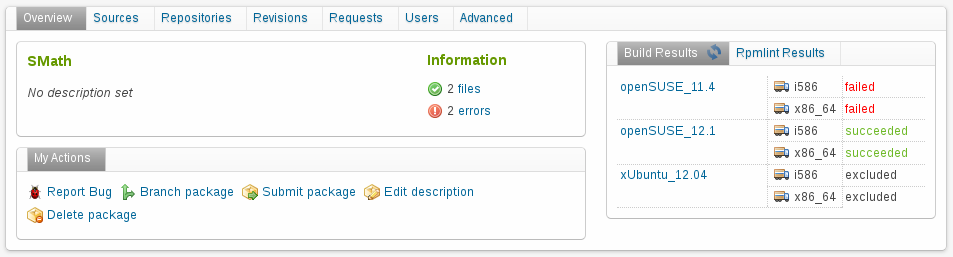
\includegraphics[width=0.75\textwidth]{image/standard/build/opensuse-project-package.png}
\caption[برگه مدیریت پرونده‌ها در کارگزار ساخت \lr{OpenSUSE}]{
	توصیف بسته
}
\label{image/standard/build/opensuse-project-package}
\end{figure}

کارگزار ساخت بسته‌های نرم‌افزاری را مبتنی بر کدهای منبعی ایجاد می‌کند که در بسته
تعریف شده‌اند. گرچه بارگزاری کد منبع به صورت دستی در این کارگزار ممکن است اما
استفاده از سرویس‌های کد منبع روش‌های مناسب‌تری برای این کار فراهم کرده است. برای
نمونه حالتی را فرض کنید که نیاز به دریافت کد منبع از یک سرویس کنترل نسخه باشد و
یا حالتی که در آن می‌بایست پیش از ترجمه برنامه‌ها تغییرات خاصی در آنها ایجاد
شود. در سرویس‌های کد منبع این موارد پیش‌بینی شده و ابزارهای مناسبی برای مدیریت
کدهای منبع ایجاد شده است.

سرویس‌های کد منبع در حقیقت دسته‌ای از وظایف است که کارگزار ساخت پیش از آغاز
فرآیند ساخت آنها را اجرا می‌کند. سرویس‌های کد منبع می‌تواند از دانلود کد منبع تا
اعمال \lr{Patch} به روی کدهای منبع متفاوت باشد. کارگزار ساخت تنها زمانی فرآيند
ایجاد را اجرا می‌کند که تمام سرویس‌های کد منبع به صورت کامل و بدون اشکال اجرا
شود.

علاوه بر کدهای منبع، نپشته‌های مورد استفاده در ساخته بسته‌های نرم‌افزاری نیز
باید به عنوان کد منبع در کارگزار بارگزاری شود. کارگزار ساخت با استفاده از این
بپشته‌ها بسته‌های نرم‌افزاری را ایجاد و در مخزن‌های مربوطه بارگزاری می‌کند.
گرچه نپشته‌های ساخت می‌بایست از استانداردهای خاص برای ایجاد بسته استفاده کنند
اما این کارگزار از قالب‌های متفاوتی برای ایجاد بسته‌ها استفاده می‌کند. یک روش
مناسب برای ایجاد بسته‌ها استفاده از برنامه‌های \lr{spec} است که در مدیریت
بسته‌های کلاه قرمز معرفی شده است. 

در این روش علاوه بر کدهای منبع، پرونده‌های \lr{spec} برای ایجاد بسته‌های
نرم‌افزاری بارگزار می‌شود و در نهایت کارگزار ساخت با استفاده از همین کدها
بسته‌های نرم‌افزاری ار ایجاد می‌کند. کارگزار برای ایجاد بسته‌های نرم افزاری
توزیع \lr{OpenSUSE} از این روش به صورت پیش فرض استفاده می‌کند از این رو در این
بخش تنها همین روش برای ایجاد بسته‌ها مورد استفاده قرار خواهد گرفت.

در اینجا تنها فرآیند ساخته بسته‌های مستند فنی برای توزیع \lr{OpenSUSE} مورد بحث
قرار می‌گیرد که در و همانطور که اشاره شد برای ایجاد بسته مستند فنی از کدهای
\lr{spec} استفاده خواهد شد.

برای نمونه فرض کنید که بسته مورد نظر، \lr{SMath}‌ باشد که در بخش پیش مورد بحث
قرار گرفت. برای ایجاد مستند فنی این بسته با استفاده از این کارگزار در پروژه خانه
ابتدا باید یک بسته ایجاد شود. نام این بسته را نیز همنام با بسته نرم‌افزاری در
نظر گرفته می‌شود. در گام بعد کد منبع به صورت دستی بارگزاری می‌شود. با تعیین
نپشته‌های \lr{spec} کارگزار ساخت فرآیند ساخت بسته را اجرا خواهد کرد و بسته‌های
ایجاد شده را در مخزن‌ها قرار می‌دهد.

\subsection{بسته مستقل}

کارگزار ساخت \lr{OpenSUSE} توانایی اجرای چندین پرونده \lr{spec} را در هر بسته
فراهم کرده است از این رو استفاده از پرنده‌های \lr{spec} برای کارهای متفاوت نه
تنها اشکالی را ایجاد نمی‌کند بلکه به عنوان یک مزیت تلقی می‌شود. گرچه استفاده از
\lr{spec} متفاوت به صورت دستی منجر به ناهماهنگی و سربار در فرآیند ساخت می‌شود
اما در کارگزار ساخت منجر به واضح بودن فرآیندهای ساخت و سادگی آنها می‌شود.

در اینجا نیز مانند روشی که در \lr{RPM} دنبال شد، یک پرونده \lr{spec} ایجاد
می‌شود و فرآیند ساخت بسته به صورت کامل در آن تشریح می‌شود. این پرونده تمام اصول
تعریف شده در \lr{RPM} را در برداشته و از همان روش برای ایجاد بسته‌های نرم افزاری
استفاده می‌کند.

اما نکته‌ای که باید همواره در استفاده از \lr{spec} در کارگزار ساخت مورد توجه قرا
گیرد تعیین بسته‌هایی است که در فرآیند ساخت مورد نیاز است. کارگزار همواره یک
ماشین مجازی را برای ایجاد بسته‌ها ایجاد می‌کند و فرآیند ساخت را مبتی بر آن انجام
می‌دهد. این ماشین مجازی با استفاده از حداقل بسته‌های مورد نیاز بارگزاری می‌شود
از این رو نیاز است که بسته‌ها و ابزارهای مورد نیاز در فرآیند ساخت تعیین شود.

گرچه تعیین بسته‌های مورد نیاز در فرآیند ساخت ممکن است در دید نخست دشوار به نظر
برسد اما این کار با استفاده از \lr{spec} به سادگی قابل انجام است. در این پرونده
با استفاده از برچسب \lr{BuildRequires} می‌توان تمام بسته‌های مورد نیاز برای
فرآیند ساخت را تعیین کرد. این برچسب در قسمت خوصیت‌های عمومی \lr{spec} قرار
می‌گیرد. برای نمونه اگر در فرآیند ساخت نیاز به استفاده از بسته نرم‌افزار \lr{A}
باشد با اضافه کردن کد زیر به پرونده \lr{spec} می‌توان از نصب بودن این بسته پیش
از آغاز شدن فرآیند ساخت اطمینان حاصل کرد.

\begin{latin}
\lstset{language=C++}
\begin{lstlisting}[frame=single]
BuildRequires: A
\end{lstlisting}
\end{latin}

بدیهی است که در فرآیند ساخت مستند فنی نیاز به استفاده از ابزار \lr{Doxygen} است.
از این رو دور از انتظار نیست که در پیش از آغاز فرایند ساخت نیاز به نصب و راه
اندازی این بسته باشد.

نکته‌ای که باید در نظر داشت این است که ممکن است خود ابزارهای مورد نیاز در فرآیند
نصب نیز به بسته‌های دیگری برای اجرا نیاز داشته باشند! در این حالت چه باید کرد؟
کارگزار ساخت فرآیند نصب بسته‌های مورد نیاز را با استفاده از مدیریت بسته‌های
مانند مدیریت بسته‌های کلاه قرمز یا \lr{RPM} انجام می‌دهد، بنابراین سیستم به صورت
خودکار نه تنها بسته مورد نیاز بلکه تمام بسته‌های مورد نیاز دیگر ار نصب خواهد
کرد.

از دیگر بسته‌های مورد نیزا در فرآیند ساخت می‌توان به \lr{texlive} اشاره کرد.
\lr{Doxyge} با استفاده از ابزارهای معرفی شده در این بسته رابطه‌های ریاضی را
ایجاد می‌کند و در نهایت مستند فنی در قالب چاپی را نیز با همین ابزار ایجاد
می‌کند. اما خود بسته \lr{Doxygen} به این بسته وابسته نیست، بنابر این اگر این
بسته به عنوان بسته مورد نیاز در فرآیند ایجاد معرفی نشود، فرآیند ایجاد مستند فنی
با مشکل روبرو خواهد شد.

در گفتارهای پیشین ابزارهای متفاوتی به عنوان ابزارهای مورد استفاده در
\lr{Doxygen} معرفی شده است که می‌تواند در فرآیند ساخت مورد استفاده قرار گیرد. از
این رو پیش از فرآیند ساخت می‌بایست از نصب بودن آنها اطمینان حاصل کرد. البته
استفاده از این بسته‌ها به تنظیم‌های موجود در پرونده پیکره بندی مستند فنی
وابسته‌ است.

برای نمونه در ایجاد مستند فنی \lr{SMath} ابزارهای مورد نیاز به صورت زیر تعیین
شده است که شامل تمام ابزارهای مورد نیاز برای ساخت یک مستند فنی کامل است.


% TODO: maso 1391: تعیین بسته‌های مورد نیاز
% برای نصب کامل یک سیستم به بسته‌های متفاوتی نیاز است که از آنها در ترسیم و یا
% سازماندهی کردن مستند استفاده می‌شود. از این رو نیاز است که این بسته‌ها به صورت
% کامل و دقیق برای مستند سازی تعیین شود.

\begin{latin}
\lstset{language=C++}
\begin{lstlisting}[frame=single]
BuildRequires: texlive texlive-bin texlive-fonts-extra texlive-xetex 
graphviz doxygen
\end{lstlisting}
\end{latin}

با ایجاد این تغییرها و اضافه کردن پرونده \lr{spec} سرور ساخت فرآیند ایجاد را
زمان بندی کرده و در موقعیت مناسب اجرا می‌کند. در نهایت نتیجه به دست آمده در
فهرست بسته‌های موجود مخزن‌های نرم‌افزاری ایجاد شده قرار می‌گیرد و کاربران می‌توانند
از آنها استفاده کنند.

\subsection{زیر بسته مستند فنی}

همانند روش زیر بسته که در بخش  \lr{RPM} معرفی شد، در اینجا نیز می‌توان با
استفاده از یک پرونده \lr{spec} نه تنها برنامه‌های ایجرایی بلکه مستندهای فنی را
نیز ایجاد کرد. تنها تفاوت مهمی که در اینجا نیاز است تعیین بسته‌هایی است که در
فرآیند ساخت مورد نیاز است.

بسته‌های مورد نیاز در فرایند ساخت ممکن است برای هر زیر بسته متفاوت باشد با این
وجود تمام بسته‌های مورد نیاز در بخش اصلی معرفی می‌شود. از این رو برای ایجاد زیر
بسته مستند فنی می‌بایست پیش از هر چیز ابزارهای مورد نیاز را تعیین کرد. در تکه کد
زیر روش تعیین ابزارهای مورد نیاز آورده شده است.

\begin{latin}
\lstset{language=C++}
\begin{lstlisting}[frame=single]
BuildRequires: gcc make automake libqt4-devel ... doxygen ...
\end{lstlisting}
\end{latin}

با اضافه کردن ابزارها و بارگزار پرونده \lr{spec}، کارگزار علاوه بر ایجاد
بسته‌های نرم‌افزار بسته مستند فنی را نیز ایجاد خواهد کرد.

% %
% حق نشر 1390-1402 دانش پژوهان ققنوس
% حقوق این اثر محفوظ است.
% 
% استفاده مجدد از متن و یا نتایج این اثر در هر شکل غیر قانونی است مگر اینکه متن حق
% نشر بالا در ابتدای تمامی مستندهای و یا برنامه‌های به دست آمده از این اثر
% بازنویسی شود. این کار باید برای تمامی مستندها، متنهای تبلیغاتی برنامه‌های
% کاربردی و سایر مواردی که از این اثر به دست می‌آید مندرج شده و در قسمت تقدیر از
% صاحب این اثر نام برده شود.
% 
% نام گروه دانش پژوهان ققنوس ممکن است در محصولات دست آمده شده از این اثر درج
% نشود که در این حالت با مطالبی که در بالا اورده شده در تضاد نیست. برای اطلاع
% بیشتر در مورد حق نشر آدرس زیر مراجعه کنید:
% 
% http://dpq.co.ir/licence
%
\section{\lr{Bamboo}}

\lr{Bamboo} یک کارگزار مجتمع سازی پیوسته\LTRfootnote{Continuous Integration} یا
\lr{CI} است که می‌تواند برای توسعه سیستم‌های نرم‌افزاری و ساخت آنها بر اساس
قراردادهای این روش مورد استفاده قرار گیرد.

% What does this mean?
مجتمع سازی پیوست یک متدلوزی توسعه و ساخت سیستم‌های نرم‌افزاری است که در آن 
هم زمان با تغییر کد منبع سیستم‌های نرم‌افزاری، فرآیند ترجمه، ارزیابی
برنامه‌ها و ارزیابی مجتمع سازی اجرا (و یا تحریک) می‌شود تا از درست بودن کدهای
ایجاد شده در مقایسه با کل سیستم اطمینان حاصل شود. در این فرآیند توسعه همواره
کیفیت نرم‌افزار ایجاد شده در حالت کلی و ایجاد بسته‌های نرم‌افزاری در قبال هر
تغییر بررسی خواهد شد. شکل \ref{image/standard/build/bamboo-arch} فرآیند کلی مورد
استفاده در این متدلوژی را نمایش داده است.

فرآیند ایجاد سنتی سیستم‌های نرم‌افزاری شامل ترجمه، ارزیابی برنامه‌ها و ایجاد
بسته‌ها همواره در این متدلوژی اجرا می‌شود اما به این معنی نیست که به واسطه هر
تغییر یک نسخه جدید از نرم‌افزار ایجاد شده است. از این رو فرآیند ایجاد نسخه جدید
از یک سیستم نرم‌افزاری کمی با حالت سنتی آن متفاوت است. در این متدلوژی ارائه یک
نسخه جدید تنها زمانی انجام می‌شود که تمام نقشه راه در نظر گرفته شده برای سیستم
نرم‌افزاری به صورت کامل پیاده سازی شده و تمام ارزیابی‌ها را با موفقیت پشت
سر گذاشته باشد.

\begin{figure}
\centering
\includegraphics[width=0.75\textwidth]{image/standard/build/bamboo-arch}
\caption[فرآیند مجتمع سازی پیوسته یا \lr{CI}]{
	در این فرآيند
}
\label{image/standard/build/bamboo-arch}
\end{figure}


% How does Bamboo do this?

% Bamboo is the central management server which schedules and coordinates all work.
اما بامبو یک کارگزار مرکزی است که تمام فرآیندهای ساخت و ارزیابی بسته‌های
نرم‌افزاری ایجاد شده را مدیریت و برنامه ریزی می‌کند. این کارگزار با استفاده از
زیر سیستم‌های موجود، نرم‌افزارهای متفاوت را ترجمه کرده و ارزیابی‌های تعریف شده
برای آنها را اجرا می‌کند.

% Bamboo itself has interfaces and plugins for lots of types of work.
گرچه افزونه‌های متفاوتی برای این کارگزار تعریف شده است که قادر هستند کارهای
متفاوتی را در فرآیند ساخت و ارزیابی اجرا کنند اما امکان تعریف افزونه‌های جدید
نیز پیش بینی شده است. توانایی تعریف افزونه‌های جدید برای این کارگزار، آن را به
عنوان یک ابزار بسیار قدرتمند در متدلوژي مجتمع سازی پیوسته تبدیل کرده است.

%  Bamboo first gets your source from a source repository (lots of plugins here for a variety of systems).
فرآیند کلی ایجاد و ارزیابی سیستم‌های نرم‌افزاری با دریافت برنامه‌های ایجاد شده
از سرورهای کنترل نسخه آغاز می‌شود. این کارگزار با استفاده از افزونه‌های متفاوت
توانایی دریافت برنامه‌های منبع از کارگزارهای متفاوت کنترل نسخه مانند \lr{Git}،
\lr{SVN}، \lr{CVS} و غیر را دارد.

% Then Bamboo starts the build - that can be done by calling something like MSBuild to build your Visual Studio solution, or Maven to call your compiler and linker - whatever you use.
فرآیند ساخت در این کارگزار با فراخوانی ابزارها معمول ساخت برنامه‌های نرم‌افزاری
اینجام می‌شود. برای نمونه با استفاده از فراخوانی مترجم \lr{GCC} در لینوکس
نرم‌افزارهایی که به زبان برنامه سازی \lr{C/C++} ایجاد شده‌اند ترجمه می‌شوند. از
این رو زیر سیستم‌های تعریف شده برای این کارگزار می‌بایست توانایی استفاده از این
فراخوانی‌های در آنها ایجاد شده باشد (به این معنی  نه تنها ابزارهای مورد نیاز
باید نصب شده باشد بلکه در مسیرهای پیش فرض سیستم قرار گرفته شده باشد).

% Once your solution or project is built, you have "artifacts" (build results, for example, an executable app, config files, etc.).
پس از اتمام فرآیند ساخت گردایه‌ای از برنامه‌های و پرونده‌هایی ایجاد خواهد شد که
به عنوان نتیجه ساخت در نظر گرفته می‌شود. نتیجه‌های ایجاد شده در فرآیند ساخت را
اصطلاحا مصنوع\LTRfootnote{Artifact} گفته می‌شود. مصنوعات ایجاد شده در فرآیند
ساخت ممکن است از یک برنامه‌اجرایی تا یک پرونده پیکره بندی متفاوت باشد. برای
نمونه مستند فنی که نتیجه فرآیند ساخت مستند بر اساس کد فنی است شامل پرونده‌های
زنگام\LTRfootnote{HTML}، تصاویر و پوشه‌های متفاوت است.

% You can do additional things with the build artifacts:
%         zip them up into a ZIP file and copy them somewhere.
%         run a install builder on them and create an MSI.
%         install them on a test server to make sure everything installs just fine.
کارگزار ساخت می‌تواند کارهای متفاوتی را بر اساس مصنوعات انجام دهد. فشرده سازی،
نصب، اجرا برنامه‌های ارزیاب بخشی از فرآیندهایی است که می‌توان بر اساس مصنوعات
اجرا کرد. برای نمونه با نصب یک برنامه ایجاد شده به روی ماشین‌های مجازی در نظر
گرفته شده، درست بودن فرآیند نصب مورد بررسی قرار می‌گیرد.

% Bamboo provides a web front-end for configuration and for reporting the status of builds.
استفاده از یک تارافزار به عنوان واسط کاربر بامبو را به یک کارگزار بسیار ساده
تبدیل کرده است که با وجود سادگی ظاهر توانایی اجرای فرآیندهای ساخت بسیار پیچیده
را دارد. با استفاده از این واسط کاربر به سادگی می‌توان نتایج به دست آمده از
فرآیندهای ساخت متفاوت را بررسی و تنظیم‌های مورد نیاز را در پروژه‌های ایجاد کرد.
 
% What does Bamboo need?
کارگزار بامبو با زمانبندی فرآیند ساخت هر نرم‌افزار، فرآیندهای ارزیابی را به روی
نتایج به دست آمده از آن را اجرا خواهد کرد. اما برای استفاده از تمام امکانهای
تعریف شده در این کارگزار نیاز است که پیش نیازهای آن فراهم شود. تمام نیازهای این
کارگزار در این فرآیند به عبارت است از:

\begin{itemize}
  \item کارگزار کنترل نسخه و کد منبع
  \item نپشته‌های ایجاد
  \item برنامه‌های ارزیابی
  \item نپشته‌های بسته بندی
  \item نپشته‌های ارزیابی مجتمع سازی
\end{itemize}

در متدلوژی مجتمع سازی پیوست فرض بر این است فردی که کد منبع را تغییر می‌دهد
مسئولیت تمام تغییرهایی خواهد بود که در کل سیستم رخ می‌دهد. این فرد می‌بایست تمام
اشکالهای احتمالی که ممکن است در کل سیستم رخ دهد را برطرف کرده تا فرآیند ساخت به
صورت کامل اجرا شود و مصنوعات ایجاد شده ارزیابی‌های تعریف شده را با موفقیت طی
کند.

نکته‌ای که باید به آن توجه کرد این است که زیر سیستم‌های مورد استفاده در فرآیند
ساخت و ارزیابی توانایی‌های خاص خود را دارند از این رو برای ایجاد نپشته‌های ساخت
و ارزیابی می‌بایست توانایی‌های مورد نیاز به درستی تعیین شود. از این رو کارگزار
تنها زمانی که زیر سیستم مناسب برای اجرای این فرایند را در اختیار داشته باشد به
اجرای نپشته‌های ساخت و ارزیابی خواهد پرداخت.

% How is a Bamboo workflow organised?

کارگزار بامبو، وظایف مورد نیاز در فرآیند مجتمع سازی را با استفاده از موجودیت‌های
متفاوتی مانند پروژه، نقشه، کار و وظیفه سازماندهی می‌کند. ساختار سلسله مراتبی این
موجودیت ها در شکل \ref{image/standard/build/bamboo-workflow-objects} نمایش داده
شده است.

در فرآیند ایجاد یک پروژه ابتدا کارگزار نخستن نقشه را انتخاب می‌کند و به اجرا آن
می‌پردازد. پس از پایان یافتن هر نقشه، نقشه بعد برای اجرا انتخاب خواهد شده در
حالی که هر نقشه نیز خود از چندین وهله تشکیل شده است. از این رو برای اجرا هر وهله
نیاز است تمام کارهای تعریف شده در آن به ترتیب اجرا شود. برای اجرای هر کار نیز
نیاز است که وظایف تعریف شده در آن به ترتیب اجرا شود. بنابر این برای اجرای هر
نقشه از یک پروژه نیاز است تمام وظیفه‌ها، کارها و وهله‌ها به صورت کامل اجرا شوند
تا آن نقشه تکمیل شود.


\begin{figure}
\centering
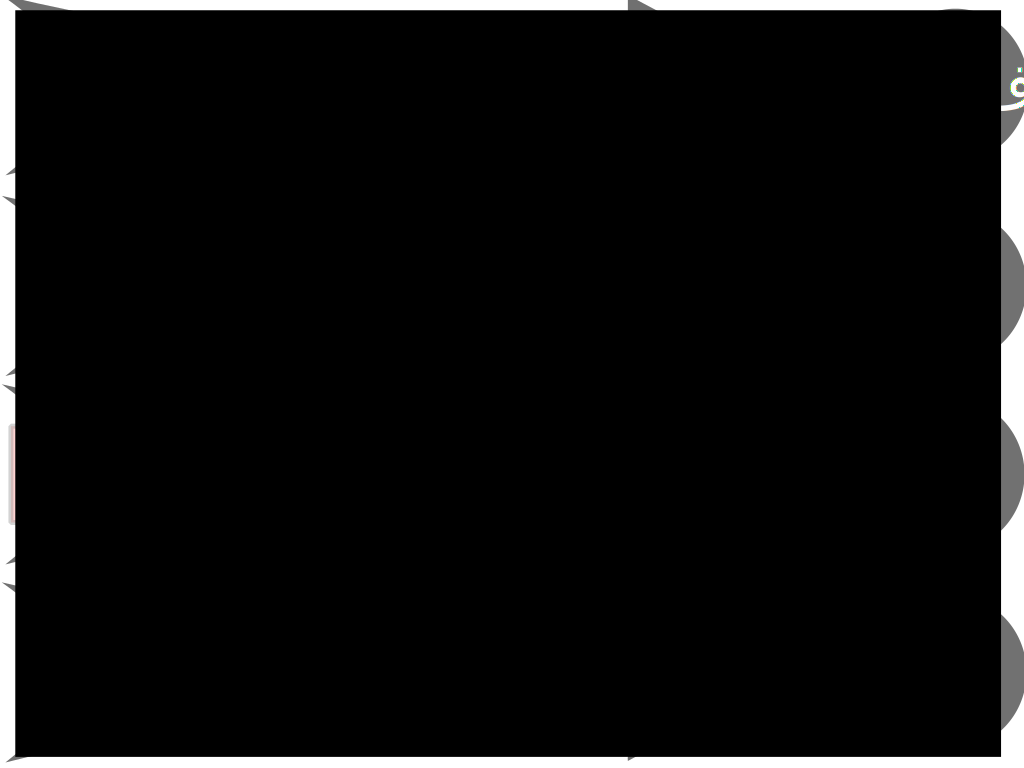
\includegraphics[width=0.75\textwidth]{image/standard/build/bamboo-workflow-objects}
\caption[فرآیند مجتمع سازی پیوسته یا \lr{CI}]{
	در این فرآيند
}
\label{image/standard/build/bamboo-workflow-objects}
\end{figure}


% Project	
% 
%     Has one, or more, plans.
%     Provides reporting (using the wallboard, for example) across all plans in the project.
%     Provides links to other applications.
% 
% Plan	
% 
%     Has a single stage, by default, but can be used to group jobs into multiple stages.
%     Processes a series of one or more stages that are run sequentially using the same repository.
%     Specifies the default repository.
%     Specifies how the build is triggered and triggering dependencies between a plan and other plans in the project.
%     Specifies notifications of build results.
%     Specifies who has permission to view and configure the plan and its jobs.
%     Provides for the definition of plan variables.
% 
% Stage	
% 
%     Has a single job, by default, but can be used to group multiple jobs.
%     Processes its jobs in parallel, on multiple agents (where available).
%     Must successfully complete all its jobs before the next stage in the plan can be processed.
%     May produce artifacts that can be made available for use by a subsequent stage.
% 
% Job	
% 
%     Processes a series of one or more tasks that are run sequentially on the same agent.
%     Controls the order in which tasks are performed.
%     Collects the requirements of individual tasks in the job, so that these requirements can be matched with agent capabilities.
%     Defines the artifacts that the build will produce.
%     Can only use artifacts produced in a previous stage.
%     Specifies any labels with which the build result or build artifacts will be tagged.
% 
% Task	
% 
%     Is a small discrete unit of work, such as source code checkout, executing a Maven goal, running a script, or parsing test results.
%     Is run sequentially within a job on a Bamboo working directory.
    
    
    
\subsection{کار مستند فنی}

ایجاد مستند فنی را می‌توان در قالب یک کار در این کارگزار در نظر گرفت. در این کار
ابتدا باید کد منبع از مخزن‌های کنترل نسخه دریافت شده و بر اساس آن مستند فنی
ایجاد شود. در نهایت مستند فنی ایجاد شده به صورت پرونده‌های فشرده ایجاد شود و به
عنوان مصنوعات در سیستم معرفی شود.


ایجاد پروژه

ایجاد نقشه

ایجاد وهله

ایجاد کار 



\subsubsection{کد منبع}

کد منبع از منبع کنترل نسخه دریافت می‌شود

\subsubsection{مستند فنی}

مستند فنی بر اساس آن ایجاد  می‌شود

\subsubsection{بسته بندی}

نتایج به دست آمده بسته بندی می شود



% TODO : مصطفی ۱۳۹۰-۱۲ : استاندارد جاوا در نسخه اول وارد نمی‌شود.
%\input{استانداردها/استاندارد-جاوا}
